% Préambule
\documentclass[oneside, a5paper, 12pt]{book}
% Configuration des marges
\usepackage[margin=0.8in]{geometry} % Définit les marges du document

% Personnalisation des titres de section et table des matières
\usepackage{sectsty, tocloft, hyperref} % Importe les packages nécessaires pour personnaliser les titres et la table des matières
\hypersetup{
    pdfauthor={Kevin Delfour}, % Définit l'auteur du PDF
    pdftitle={L'envers du décor des Entreprises libérée}, % Définit le titre du PDF
    pdfkeywords={entreprise, libérées, utopie, envers, décor}, % Définit les mots-clés du PDF
    hidelinks % Cache les liens dans le PDF
}

% Cadres, tailles de police et en-têtes/pieds de page personnalisés
\usepackage{framed, anyfontsize, fancyhdr} % Importe les packages nécessaires pour personnaliser les cadres, les tailles de police et les en-têtes/pieds de page

% Police Garamond et paramètres de langue
\usepackage{ebgaramond, float} % Importe la police Garamond et le package float pour la gestion des flottants
\usepackage[french]{babel} % Définit le français comme langue principale
\usepackage[T1]{fontenc} % Utilise la codification de caractères T1

% Couleurs personnalisées et graphiques TikZ
\usepackage[dvipsnames]{xcolor} % Importe le package xcolor avec les noms de couleurs dvips
\usepackage{tikz, microtype, GS1, qrcode} % Importe les packages nécessaires pour les graphiques TikZ, la microtypographie, les codes-barres GS1 et les QR codes
\usetikzlibrary{calc} % Utilise la bibliothèque calc de TikZ pour les calculs de coordonnées

\usepackage[labelformat=empty]{caption} % Importe le package caption avec un format de label vide
\captionsetup{justification=raggedleft, font={tiny, color=gray}, singlelinecheck=false} % Configure les légendes des figures

% Contenu : texte aléatoire, boucles, images et commandes supplémentaires
\usepackage{lipsum, pgffor, graphicx, etoolbox} % Importe les packages nécessaires pour le contenu : texte aléatoire, boucles, images et commandes supplémentaires

% Configuration de la mise en page
\renewcommand{\familydefault}{\sfdefault} % Utilise la police sans serif par défaut
\setlength{\parskip}{\baselineskip} % Définit l'espacement entre les paragraphes
\setlength{\parindent}{0pt} % Supprime l'indentation des paragraphes

% Configuration de la table des matières
\setcounter{tocdepth}{2} % Définit la profondeur de la table des matières
\renewcommand{\cftpartfont}{\normalfont\bfseries\Large} % Configure la police des parties dans la table des matières
\renewcommand{\cftchapfont}{\normalfont\bfseries} % Configure la police des chapitres dans la table des matières
\renewcommand{\cftsecfont}{\normalfont} % Configure la police des sections dans la table des matières
\renewcommand{\cftsubsecfont}{\normalfont} % Configure la police des sous-sections dans la table des matières
\renewcommand{\cftsubsubsecfont}{\normalfont\small} % Configure la police des sous-sous-sections dans la table des matières

% Configuration des en-têtes et pieds de page personnalisés
\pagestyle{fancy} % Utilise le style de page fancy
\fancyhead{} % Supprime l'en-tête par défaut
\fancyhead[LO, L]{ \color{gray}\scriptsize\leftmark} % Configure l'en-tête gauche
\fancyfoot{} % Supprime le pied de page par défaut
\fancyfoot[R]{\scriptsize\thepage} % Configure le pied de page droit
\renewcommand{\headrulewidth}{0pt} % Supprime la ligne sous l'en-tête

\newcommand{\listfootnotesname}{Liste des sources}% 'List of Footnotes' title
\newlistof[chapter]{footnotes}{fnt}{\listfootnotesname}% New 'List of...' for footnotes

\newcommand{\insertImage}[2]{
    \markboth{}{} % Supprime les marques de tête
    \begin{figure}[H]
        \center % Centre l'image
        \includegraphics[keepaspectratio, width=\textwidth, height=\textheight]{images/#1} % Insère l'image
        \captionsetup{justification=raggedright, singlelinecheck=false} % Aligne la légende sur la gauche
        \caption{#2} % Ajoute une légende à l'image
    \end{figure}
    \newpage % Crée une nouvelle page après l'image
}

\makeatletter
\renewcommand{\thefigure}{\@arabic\c@figure}
\makeatother


\let\oldfootnote\footnote % Save the old \footnote{...} command
\renewcommand\footnote[1]{
    \oldfootnote{#1}% Make a regular footnote with added margin.
    \addcontentsline{fnt}{footnotes}{\protect
        \numberline{\thepart.\thefootnotes}\hspace{1,8em}#1}% Add the 'List of...' entry with a margin between the number and the note, and include the part number in the numbering.
}

\makeatletter
\@addtoreset{chapter}{part} % Réinitialise le compteur de chapitres à chaque nouvelle partie
\makeatother

% Commandes personnalisées
\newcommand{\subtitle}{L'envers du décor}
\newcommand{\edition}{2023}

% Informations sur le document
\title{L'envers du décor des Entreprise libérée}
\author{Kevin Delfour}
\date{\today}

% Début du document
\begin{document}

% Introduction
% 1. Présentation du concept d'entreprise libérée
% a. Définition et origines
% b. Principes et valeurs
% c. Exemples d'entreprises libérées

% Partie I : Les défis et problèmes liés à l'organisation des entreprises libérées
% 1. La communication et la prise de décision
% a. La difficulté de trouver un équilibre entre autonomie et cohésion
% b. Les risques de désorganisation et de confusion
% c. Les outils et méthodes pour faciliter la communication et la prise de décision
% 2. La gestion des ressources humaines
% a. Le recrutement et l'intégration des nouveaux employés
% b. La formation et le développement des compétences
% c. La gestion des conflits et des problèmes personnels
% 3. La performance et la rentabilité
% a. La mesure de la performance dans une entreprise libérée
% b. Les risques de perte de compétitivité et de rentabilité
% c. Les stratégies pour maintenir et améliorer la performance

% Partie II : Les échecs et les leçons tirées des entreprises libérées
% 1. Les causes des échecs
% a. Les erreurs de mise en œuvre et de gestion
% b. Les résistances internes et externes
% c. Les limites du modèle d'entreprise libérée
% 2. Les leçons tirées des échecs
% a. L'importance de l'adaptation et de la flexibilité
% b. La nécessité d'un leadership fort et d'une vision claire
% c. La prise en compte des spécificités de chaque entreprise

% Partie III : Les réfractaires au modèle d'entreprise libérée et leurs arguments
% 1. Les critiques du modèle d'entreprise libérée
% a. Les arguments économiques et financiers
% b. Les arguments sociaux et culturels
% c. Les arguments liés à la gouvernance et à la gestion
% 2. Les alternatives au modèle d'entreprise libérée
% a. Les autres formes d'organisation et de management
% b. Les innovations et les expérimentations en cours
% c. Les perspectives d'évolution du modèle d'entreprise libérée

% Partie IV : L'expérience humaine dans les entreprises libérées

% 1 : Les expériences des employés
% a. L'impact de l'autonomie sur l'engagement des employés
% b. Gestion des défis et des conflits dans un environnement de travail libéré
% c. Témoignages d'employés et études de cas
% 2 : Le rôle des leaders dans les entreprises libérées
% a. Redéfinir le leadership dans une entreprise libérée
% b. Défis et récompenses du leadership libéré
% c. Témoignages de leaders et études de cas
% 3 : Les impacts sur les parties prenantes externes
% a. Relation avec les clients dans une entreprise libérée
% b. Relation avec les fournisseurs et les partenaires commerciaux
% c. Impact sur la communauté locale et la société en général

% Conclusion
% 1. Les enseignements à tirer pour les entreprises libérées et les autres organisations
% 2. Les pistes de réflexion pour l'avenir des entreprises libérées et du management en général

% Front matter
\frontmatter

    % Cover
    \newpage
% ---- Couverture
% Insert the image as the background for the cover page
\begin{tikzpicture}[overlay,remember picture]
    \node[inner sep=0pt, anchor=south west] at (current page.south west) {
        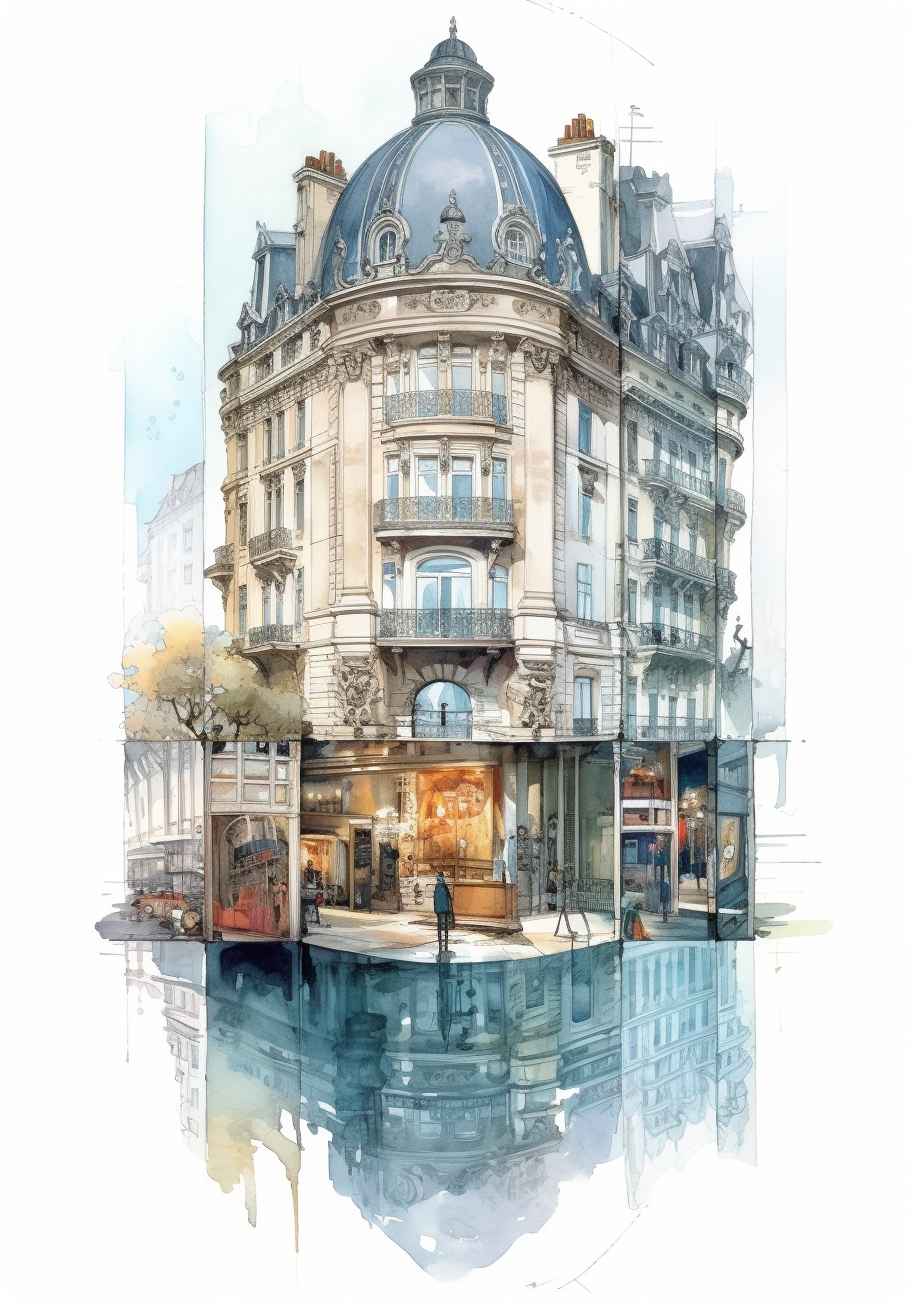
\includegraphics[keepaspectratio, width=\paperwidth]{images/375669df-73f6-4168-9295-19bef29746b5.png}
    };

    % White frame with 0.33 opacity
    \fill[white, opacity=0.33] (current page.south west) rectangle (current page.south east |- current page.center);

    % Title
    \node[align=center] at ($(current page.center)+(0,-5.5)$)
    {
    {\fontsize{45}{72} \fontfamily{cmr}\selectfont \textcolor{black}{\textbf{L'envers du décor}}}\\[0.5cm]
    {\fontsize{30}{72} \fontfamily{cmr}\selectfont \textcolor{black}{\textbf{des Entreprises}}}\\[0.25cm]
    {\fontsize{45}{72} \fontfamily{cmr}\selectfont \textcolor{black}{\textbf{Libérées}}}
    };

    % Author
    \node[align=center] at ($(current page.center)+(0,-10)$)
    {
        {\fontsize{12}{19.2} \textcolor{black}{\selectfont {Kevin Delfour}}}\\[3pt]
    };
\end{tikzpicture}

\newpage
\thispagestyle{empty} % Supprime les en-têtes et pieds de page sur cette page
\mbox{}
% Page blanche

%=========================================
\newpage{}
\thispagestyle {empty}
\begin{titlepage}
    \centering
    \vspace*{3cm}
    {\fontsize{40}{72} \fontfamily{cmr}\selectfont \textcolor{black}{\textbf{L'envers du décor}}}\\[0.5cm]
    {\fontsize{30}{72} \fontfamily{cmr}\selectfont \textcolor{black}{des Entreprises}}\\[0.25cm]
    {\fontsize{40}{72} \fontfamily{cmr}\selectfont \textcolor{black}{Libérées}}\\[2cm]
    {\fontsize{12}{19.2} \textcolor{black}{\selectfont {Kevin Delfour}}}\\[3pt]
    \vfill
\end{titlepage}

%=========================================
\newpage{}
\thispagestyle {empty}
\vspace*{\fill}

\begin{flushleft}

    \textbf{L'envers du décor des Entreprises Libérées}, © Kevin Delfour, 2023 \\[0.25cm]
    \textbf{ISBN : } xxx xxx xxx xx

    \noindent Tous droits réservés. Aucune partie de ce livre ne peut être reproduite, stockée dans un système de recherche documentaire ou transmise sous quelque forme ou par quelque moyen que ce soit, électronique, mécanique, photocopie, enregistrement ou autre, sans l'autorisation préalable écrite de l'auteur ou de l'éditeur, sauf dans le cas de brèves citations intégrées à des critiques ou des articles de presse.

    Toute violation des droits d'auteur est passible de poursuites judiciaires, y compris de réclamations en dommages-intérêts et de demandes d'injonction.

    Certaines images ont été créées en utilisant le service Midjourney par Kévin Delfour, qui détient les droits sur ces images conformément aux termes de service de Midjourney.

\end{flushleft}

%=========================================
\newpage{}
\thispagestyle {empty}

\vspace*{2cm}

\begin{center}
    \vspace*{\fill}
    \parbox{10cm}{
        \begin{center}
            \large{\selectfont
                \textit{"C'est ce que nous faisons aujourd'hui détermine ce que nous serons demain."}
            }

            \vspace{.5cm}\hfill{-- Kevin Delfour}
        \end{center}
    }
    \vspace*{\fill}
\end{center}

%=========================================
\newpage
\thispagestyle{empty} % Supprime les en-têtes et pieds de page sur cette page
\mbox{}
% Page blanche



    % Édito
    \insertImage{92b04921-76d0-42f4-a88e-21248e3e9194.png}{Aquarelle d'un globe terrestre avec des points marqués comme de petits bâtiments à différents endroits, symbolisant des entreprises libérées dans le monde entier.}

\part*{Édito}
Chers lecteurs,

Embarquons ensemble dans le dédale fascinant de l'univers entrepreneurial où, parmi les innombrables formes d'organisation, l'entreprise libérée brille comme un phare de promesses. On peut facilement être ébloui par la perspective de travailleurs autonomes, d'initiatives spontanées et d'un environnement professionnel débordant de liberté et de respect. Oui, ça sonne bien sur le papier, n'est-ce pas ?

C'est ce que j'ai longtemps cru et c'est toujours une conviction.

Mais pourquoi ecrire un livre sur les zones d'ombres d'une forme d'organisation auquel je tiens tant?

Au détour de mes discussions, j'ai eu l'occasion de rencontrer des personnes qui détestent littéralement ce mode d'organisation parceque lorsqu'on le voile du "hype" et "l'espoir d'utopiste", ce mode d'organisation révèlerait une bureaucratie qui accentue le surmenage, la discrimination et le "gaslighting" et qu'accessoirement, ce modèle n'est pas capable de passer à l'échelle.

Cette discussion m'a ouvert les yeux, non pas sur les vis cachés d'un modèle, mais sur les erreurs que l'on peut commettre pensant que ce modèle libérateur n'est pas sans risques, et comme toute mise en place d'un nouveau modèle d'organisation, il necessite de la rélféxion, de la vigilance et surtout de l'encadrement pour éviter les échecs, les erreurs et les dérives.

Comme le dit le vieil adage, toute médaille a son revers. Derrière les belles histoires, les discours inspirants et les études de cas prometteuses, se cache une réalité plus complexe et souvent plus sombre. Quelle est la véritable essence de l'entreprise libérée ? Quels sont ses principes fondateurs ? Comment est-elle gérée au quotidien ? Quels sont ses avantages et ses inconvénients ? Comment est-elle perçue par ceux qui y travaillent, ceux qui la dirigent, ceux qui la conseillent ?

Voici l'objectif de ce livre : éclairer les zones d'ombre, démystifier les clichés, comprendre les enjeux et mettre en lumière les difficultés inhérentes au modèle d'entreprise libérée. Car, chers lecteurs, il est important de comprendre que si l'entreprise libérée a le potentiel de transformer positivement la vie de travail, elle n'est pas une panacée universelle. Il n'y a pas de formule magique en matière d'organisation d'entreprise. Chaque modèle a ses forces et ses faiblesses, et il est essentiel d'aborder ces questions avec un esprit ouvert et critique.

Ce voyage vous guidera à travers les coulisses des entreprises libérées, en explorant les réalités du terrain, en analysant les réussites et les échecs, et en dévoilant les vérités qui se cachent derrière le jargon et les slogans. Nous plongerons dans le vif du sujet, en exposant les défis liés à la communication, à la gestion des ressources humaines, à la performance et à la rentabilité. Nous explorerons également les raisons des échecs, les leçons tirées, ainsi que les critiques et les alternatives à ce modèle.

Alors, préparez-vous à un voyage rempli d'histoires captivantes, de faits surprenants, d'analyses perspicaces et de réflexions profondes. Qu'il s'agisse de redéfinir votre façon de penser le travail, de remodeler votre organisation ou simplement de satisfaire votre curiosité, ce livre a quelque chose pour vous. Attachez bien vos ceintures, car nous sommes sur le point de décoller pour une exploration passionnante de l'envers du décor des entreprises libérées.

Alors installez-vous confortablement, et laissez-vous guider. Mais attention, la lecture de ce livre pourrait bien bouleverser vos convictions et changer votre regard sur le monde de l'entreprise. Vous voilà prévenus !


    % Table des matières
    \newpage
% Table des matières
\tableofcontents



    % Page blanche
    \newpage
    \thispagestyle{empty}
    \mbox{}

% Main matter
\mainmatter

    % Introduction
    \insertImage{3c1da1ab-a826-4f5f-b681-6318fb79aca0.png}{Aquarelle d'une fenêtre de bureau moderne ouverte sur un environnement luxuriant et fleuri.}


\part*{Introduction}
\addcontentsline{toc}{part}{Introduction}

\textit{Libérer l'entreprise.} Au premier abord, l'idée semble aussi radicale qu'elle est séduisante. Et pourtant, il s'agit d'une pratique de plus en plus courante dans le monde des affaires d'aujourd'hui. Les entreprises libérées, ces entités audacieuses qui cherchent à réinventer la façon dont le travail est organisé et effectué, ont fait l'objet d'une attention considérable ces dernières années. Certains voient en elles le futur du travail\footnote{Fleming, P. (2019). The Worst Is Yet to Come: A Post-Capitalist Survival Guide. Repeater Books.}, tandis que d'autres y voient une tendance de gestion passagère\footnote{Gandini, A. (2019). Labour process theory and the gig economy. Human Relations, 72(6), 1039–1056. https://doi.org/10.1177/0018726718792867}. Quoi qu'il en soit, la réalité est souvent plus nuancée.

\section*{Présentation du concept d'entreprise libérée}

\subsection*{Définition et origines}

L'entreprise libérée est un modèle organisationnel qui vise à donner aux employés la liberté et la responsabilité de prendre leurs propres décisions, dans le but de favoriser l'innovation, l'efficacité et la satisfaction au travail. Ce concept, qui remonte à plusieurs décennies, a été popularisé par le professeur Isaac Getz de l'ESCP Europe dans son livre "Freedom, Inc."\footnote{Carney, B. M., \& Getz, I. (2009). Freedom, Inc.: Free Your Employees and Let Them Lead Your Business for Greater Success. Crown Business.}.

Il n'y a pas de définition unique et universellement acceptée de l'entreprise libérée, car chaque organisation est unique et adapte le concept à sa propre situation. Cependant, la plupart des entreprises libérées partagent certaines caractéristiques communes, notamment une décentralisation de l'autorité, une communication ouverte et transparente, une confiance et un respect mutuels, et un accent mis sur l'autonomie et l'initiative individuelle.

\subsection*{Principes et valeurs}

Les principes et valeurs qui sous-tendent le modèle de l'entreprise libérée sont enracinés dans des théories et des pratiques de gestion plus larges, y compris le management participatif, la théorie X et Y de Douglas McGregor, et les principes de responsabilité et d'autonomie prônés par Peter Drucker et d'autres gourous de la gestion\footnote{Drucker, P. (1954). The Practice of Management. Harper \& Brothers.}.

Dans une entreprise libérée, les employés sont non seulement autorisés, mais encouragés à prendre des initiatives et à faire preuve de créativité. La communication est ouverte et bidirectionnelle, avec un accent mis sur le partage des informations et des connaissances. La confiance est considérée comme un élément fondamental de la culture organisationnelle, et les managers sont vus comme des facilitateurs plutôt que comme des commandants.

\subsection*{Exemples d'entreprises libérées}

Des entreprises de toutes tailles et de tous secteurs ont adopté le modèle de l'entreprise libérée. Parmi les exemples les plus connus, on trouve FAVI, une entreprise française de sous-traitance automobile dirigée par Jean-François Zobrist\footnote{Zobrist, J.-F. (2012). La belle histoire de FAVI: L'entreprise qui croit que l'homme est bon. Humanisme \& Organisations.}, et Valve, un développeur américain de jeux vidéo célèbre pour sa structure organisationnelle plate et son manque de hiérarchie formelle\footnote{Laloux, F. (2014). Reinventing Organizations: A Guide to Creating Organizations Inspired by the Next Stage of Human Consciousness. Nelson Parker.}.

Ces entreprises ont été saluées pour leur capacité à stimuler l'innovation, à améliorer la satisfaction des employés et à obtenir des résultats financiers solides. Cependant, elles ont également dû faire face à des défis importants, notamment en matière de coordination, de contrôle et de gestion du changement.

Dans ce livre, nous explorerons ces défis et les leçons que nous pouvons en tirer. Nous examinerons également les critiques et les controverses qui entourent le modèle de l'entreprise libérée, et nous envisagerons des alternatives et des perspectives d'évolution.

En fin de compte, notre objectif est de fournir une vue d'ensemble équilibrée et approfondie de ce phénomène passionnant et complexe. Nous espérons que ce livre vous aidera à comprendre ce que signifie vraiment "libérer l'entreprise" - et peut-être à déterminer si c'est une voie que vous, ou votre organisation, souhaitez emprunter.



    % Part 01
    \part{Les défis et problèmes liés à l'organisation des entreprises libérées}

Les entreprises libérées, caractérisées par leurs principes de décentralisation de l'autorité, de transparence, de confiance et de responsabilité, offrent un modèle organisationnel attrayant et prometteur. Elles représentent une rupture radicale avec les structures hiérarchiques traditionnelles, en plaçant l'individu au centre de l'organisation et en favorisant une culture d'autonomie et d'initiative.

Cependant, la mise en œuvre de ces principes n'est pas sans difficultés et défis. La transition vers une entreprise libérée nécessite une transformation profonde de la culture d'entreprise, des processus de gestion et des relations de travail. Elle implique de surmonter des obstacles institutionnels, culturels et psychologiques, et de gérer les tensions et les conflits qui peuvent surgir lors de ce processus.

Dans cette partie, nous allons explorer certains des principaux défis auxquels sont confrontées les entreprises qui cherchent à se libérer. Nous allons discuter des problèmes liés à la décentralisation de l'autorité, à la gestion de la transparence, à la construction de la confiance et à l'instauration de la responsabilité. Nous allons également examiner comment ces défis peuvent être surmontés et comment les entreprises peuvent réussir leur transition vers un modèle libéré.



    % Chapter 01
    \insertImage{fde831f5-1dd5-468b-8682-1d0e38a05cc0.png}{Aquarelle d'une réunion d'équipe dans une entreprise libérée, avec des employés partageant des idées et prenant des décisions ensemble.}

\chapter{La communication et la prise de décision}

Faites l'exercice avec moi. Dans votre entreprise, aujourd'hui, qui décide d'embaucher quelqu'un ? Qui décide d'un achat à dix mille euros ? Qui décide qu'un projet s'arrête ?

Si vous avez répondu du tac au tac, vous travaillez dans une organisation classique : la réponse, c'est un nom ou un titre, et tout le monde le connaît. Dans une entreprise libérée, ces trois questions déclenchent une conversation. Ce n'est pas un bug, c'est le principe : les décisions descendent au plus près de ceux qui font, et l'information circule à l'horizontale plutôt que de remonter et redescendre les étages\footnote{Carney, B. M., \& Getz, I. (2009). Freedom, Inc.: Free Your Employees and Let Them Lead Your Business for Greater Success. Crown Business.}.

Sur le papier, c'est plus rapide, plus intelligent, plus engageant. Dans la vraie vie, c'est tout ça — et c'est aussi le premier endroit où une libération se met à grincer. Voyons pourquoi.

\section{La difficulté de trouver un équilibre entre autonomie et cohésion}

Chez FAVI, la fonderie picarde devenue l'icône française du modèle, les opérateurs géraient leur rythme de production, leurs délais, jusqu'à l'entretien de leurs machines\footnote{Zobrist, J.-F. (2012). La belle histoire de FAVI: L'entreprise qui croit que l'homme est bon. Humanisme \& Organisations.}. Résultat : de la réactivité, de la fierté, de l'innovation. L'autonomie tient ses promesses — ce n'est pas le sujet.

Le sujet, c'est ce qui se passe quand tout le monde est autonome en même temps.

Prenez Valve, le studio américain de jeux vidéo célèbre pour son organisation sans hiérarchie : chacun choisit les projets sur lesquels il travaille, littéralement en roulant son bureau jusqu'à l'équipe de son choix\footnote{Valve Corporation (2012). Handbook for New Employees.}. C'est séduisant. C'est aussi mathématique : si chacun va vers le projet le plus excitant, qui travaille sur le projet nécessaire mais ingrat ? L'autonomie individuelle ne produit pas spontanément une cohérence collective. Personne n'a tort, chacun optimise son coin — et l'ensemble se fragmente.

Même mécanique sur les objectifs : une équipe privilégie l'innovation, une autre la réduction des coûts, et les deux ont raison localement. Sans un alignement explicite, ces bonnes décisions locales s'additionnent en incohérence globale. C'est exactement le service invisible que rendait la hiérarchie — elle alignait, souvent mal, mais elle alignait. La supprimer sans la remplacer par autre chose, c'est garder le problème et perdre la solution.

Trop de cohésion étouffe l'initiative. Trop d'autonomie dissout le collectif. Toute entreprise libérée vit sur cette ligne de crête, en permanence.

\section{Les risques de désorganisation et de confusion}

Il faut raconter l'histoire de GitHub, parce qu'elle est arrivée aux gens les plus intelligents du monde — ce qui devrait tous nous rendre modestes.

Au début des années 2010, GitHub, plateforme adorée des développeurs, fonctionne sans managers : chacun choisit son rôle et ses projets. Puis l'entreprise grandit, et les questions sans réponse s'accumulent. Qui tranche quand deux équipes veulent des choses incompatibles ? À qui parle un nouveau qui ne comprend pas où va l'entreprise ? Qui s'occupe des carrières ? En 2014, après une crise interne retentissante, GitHub réintroduit une structure de management. Non pas parce que la hiérarchie serait morale ou sacrée — mais parce que certaines fonctions qu'elle assurait n'avaient jamais été réattribuées à personne\footnote{Foss, N. J., \& Klein, P. G. (2014). Why Managers Still Matter. MIT Sloan Management Review, 56(1), 73-80.}.

La leçon n'est pas « la libération ne marche pas ». La leçon, c'est qu'une organisation sans hiérarchie a \emph{plus} besoin de clarté qu'une organisation classique, pas moins : qui est responsable de quoi, comment on tranche un désaccord, où circule l'information. Le flou n'est pas de la liberté. Le flou, c'est du pouvoir informel — celui de ceux qui parlent le plus fort, et il est bien plus difficile à contester qu'un organigramme.

Autre risque, plus prosaïque : la lenteur. Quand chaque décision exige de consulter tout le monde, on ne décide plus, on réunionne. Automattic, l'entreprise entièrement distribuée derrière WordPress, a dû construire tout un outillage — blogs internes, coordination asynchrone — pour que des centaines de personnes réparties sur la planète restent alignées sans se noyer\footnote{Mullenweg, M. (2020). The Five Levels of Autonomy. Ma.tt.}. La coordination sans hiérarchie n'est pas gratuite. Elle se paie en process, en outils et en discipline — juste ailleurs.

\section{Les outils et méthodes pour faciliter la communication et la prise de décision}

La bonne nouvelle, c'est que ces problèmes ont des solutions éprouvées. La moins bonne, c'est qu'aucune ne s'installe en cochant une case.

Côté circulation de l'information, les entreprises libérées s'appuient massivement sur l'écrit et la transparence par défaut : des outils de gestion de projet partagés, et surtout une culture où l'information est publiée plutôt que transmise. Chez Automattic, les décisions se prennent et se documentent sur des blogs internes accessibles à tous — ce qui permet à n'importe qui de comprendre pourquoi un choix a été fait, six mois plus tard, sans avoir assisté à la réunion\footnote{Berkun, S. (2013). The Year Without Pants: WordPress.com and the Future of Work. Jossey-Bass.}.

Côté décision, arrêtons-nous sur une distinction que je trouve précieuse : le consensus et le consentement, que tout le monde confond. Le consensus demande que tout le monde soit \emph{pour} — c'est épuisant, et ça donne un droit de veto au plus têtu. Le consentement, popularisé par la sociocratie puis par l'holacratie, demande seulement que personne n'ait d'objection raisonnable et argumentée\footnote{Endenburg, G. (1998). Sociocracy: The organization of decision-making, "no objection!" as the principle of sociocracy. Eburon.}. La nuance a l'air subtile ; en pratique, c'est la différence entre des décisions qui aboutissent et des réunions qui recommencent. L'holacratie pousse la logique plus loin encore, avec des rôles explicites et des rituels de décision très codifiés\footnote{Robertson, B. J. (2015). Holacracy: The New Management System for a Rapidly Changing World. Henry Holt and Co.}.

Faut-il adopter l'un de ces systèmes clés en main ? Méfiez-vous de votre premier réflexe. Ces méthodes sont des points de départ, pas des destinations : chaque entreprise qui réussit finit par les tordre pour les adapter à sa culture et à son métier. Celle qui applique le manuel à la lettre a juste remplacé son ancienne bureaucratie par une bureaucratie plus exotique.

L'outil ne fait pas la liberté. Il la rend seulement possible — le reste, c'est vous.

    % Chapter 02
    \insertImage{775323db-ad9f-460e-baa7-57c944b1bc0d.png}{Aquarelle d'un groupe de personnes accueillant à bras ouverts un nouvel arrivant dans leur équipe.}

\chapter{La gestion des ressources humaines}

Dans une entreprise classique, la fonction RH a un déroulé connu : elle recrute sur fiche de poste, forme sur catalogue, évalue sur grille et arbitre les conflits en dernier recours. On peut critiquer ce système — je ne m'en prive pas — mais reconnaissons-lui une qualité : chacun sait à quoi s'attendre.

Maintenant, retirez la hiérarchie. Qui recrute, quand il n'y a plus de « chef d'équipe » pour valider ? Qui décide qu'un salarié doit monter en compétences, quand personne n'est chargé de son évaluation ? Et surtout — on y viendra, c'est le sujet qui fâche — qui intervient quand deux personnes ne se supportent plus ?

Une entreprise libérée ne supprime pas les questions RH. Elle les redistribue. Et cette redistribution est l'un des chantiers les plus délicats de toute la transformation, parce qu'elle touche à ce qu'il y a de plus sensible : les personnes.

\section{Le recrutement et l'intégration des nouveaux employés}

Commençons par une évidence qu'on oublie systématiquement : dans une entreprise libérée, une erreur de recrutement coûte plus cher.

Dans une organisation classique, un recrutement moyen est amorti par la structure — le manager encadre, le process rattrape. Dans une entreprise libérée, la personne arrive dans un environnement qui suppose l'autonomie, l'initiative et l'adhésion à des valeurs fortes. Si le fit n'y est pas, il n'y a pas de manager pour compenser : c'est toute l'équipe qui absorbe.

C'est pourquoi les entreprises libérées confient très souvent le recrutement… aux équipes elles-mêmes. Chez Valve, les candidats sont évalués par leurs futurs pairs, autant sur leur capacité à travailler sans supervision que sur leurs compétences techniques\footnote{Valve Corporation (2012). Handbook for New Employees.}. La logique est imparable : qui est mieux placé pour choisir un coéquipier que l'équipe qui vivra avec ?

Mais recruter la bonne personne ne suffit pas — il faut réussir son atterrissage. Arriver dans une entreprise sans organigramme est une expérience déroutante : pas de chef à qui se référer, pas de parcours balisé, des codes implicites partout. Les organisations qui réussissent l'intégration l'ont comprise comme une transmission de culture, pas comme une formalité administrative. Chez Buurtzorg, l'organisation néerlandaise de soins à domicile, chaque nouvelle infirmière est formée à la philosophie de l'entreprise et au fonctionnement en équipe autogérée avant toute chose\footnote{Laloux, F. (2014). Reinventing Organizations: A Guide to Creating Organizations Inspired by the Next Stage of Human Consciousness. Nelson Parker.}. On ne lui apprend pas seulement son métier — elle le connaît déjà. On lui apprend comment on le pratique \emph{ici}.

Et l'intégration ne s'arrête pas au premier mois. Sans manager pour surveiller la trajectoire, c'est à l'équipe de vérifier régulièrement que le nouveau trouve sa place — et au nouveau d'oser demander de l'aide. Ce qui, dans une culture qui valorise l'autonomie, est moins facile qu'il n'y paraît.

% [KEVIN : comment recrutez-vous chez toi ? Un exemple de recrutement raté ou réussi à cause du "fit" vaudrait tous les paragraphes du monde.]

\section{La formation et le développement des compétences}

Dans une entreprise libérée, personne ne viendra vous inscrire à une formation. C'est à la fois la meilleure et la pire nouvelle du modèle.

La meilleure, parce que le développement autodirigé est puissant : chacun construit son parcours selon ses besoins réels — un cours en ligne, une conférence, un mentor en interne, un projet hors de sa zone de confort. Chez Morning Star, le transformateur de tomates californien souvent cité en exemple, chaque salarié est responsable de son propre développement et l'entreprise fournit les ressources\footnote{Laloux, F. (2014). Reinventing Organizations: A Guide to Creating Organizations Inspired by the Next Stage of Human Consciousness. Nelson Parker.}. Pour les profils curieux et autonomes, c'est un accélérateur formidable.

La pire, parce que ce système a un angle mort : ceux qui ne demandent rien. Dans le modèle classique, l'entretien annuel — malgré tous ses défauts — force au moins une conversation par an sur les compétences. Supprimez-le sans le remplacer, et les plus discrets peuvent passer des années sans que personne ne se penche sur leur progression. L'autodirection profite d'abord à ceux qui savent déjà se diriger. Les autres décrochent en silence.

La responsabilité de l'entreprise ne disparaît donc pas — elle se déplace. Il ne s'agit plus de prescrire des formations, mais de créer un environnement où se former est facile, visible et valorisé : du temps sanctuarisé, des ressources accessibles, des pairs qui partagent, et des rituels d'équipe où l'on parle de progression, pas seulement de production.

\section{La gestion des conflits et des problèmes personnels}

Voici le test décisif d'une entreprise libérée. Pas la stratégie, pas les outils : le premier vrai conflit.

Dans une organisation classique, le conflit a un chemin : le manager, puis les RH. Ce chemin est souvent imparfait, mais il existe. Dans une entreprise libérée, le premier réflexe est de croire que la bonne ambiance et les valeurs partagées suffiront. Elles ne suffisent jamais. Des adultes qui travaillent ensemble finissent par s'opposer — sur une décision, une charge de travail, une manière d'être. C'est la vie normale d'un collectif.

Sans mécanisme prévu, un conflit dans une entreprise libérée a un comportement particulier : il dure. Personne n'a le rôle de l'arbitre, tout le monde attend que « ça se règle entre eux », et la transparence ambiante fait que tout le monde assiste au spectacle. Ce qui aurait été une friction de bureau devient un feuilleton d'entreprise.

Les organisations matures s'outillent donc explicitement : des processus de médiation par les pairs, une escalade progressive et connue de tous — d'abord le face-à-face, puis un médiateur choisi ensemble, puis un panel — comme le pratique précisément Morning Star\footnote{Laloux, F. (2014). Reinventing Organizations: A Guide to Creating Organizations Inspired by the Next Stage of Human Consciousness. Nelson Parker.}. Chez Buurtzorg, des coachs d'équipe — qui ne sont pas des managers — aident les équipes à traverser leurs tensions sans décider à leur place. Le point commun : le chemin du conflit est défini \emph{avant} le conflit. Après, il est trop tard.

Reste les problèmes personnels — la santé, la famille, les coups durs. Une entreprise qui demande à ses salariés de s'engager en tant que personnes entières doit accepter de les soutenir en tant que personnes entières. C'est la contrepartie du modèle, et elle n'est pas optionnelle : on ne peut pas vouloir l'engagement du lundi et ignorer la détresse du jeudi.

Une entreprise libérée ne se juge pas à ses journées faciles. Elle se juge à la façon dont elle traite ses moments difficiles.

    % Chapter 03
    \insertImage{cfe76e97-852f-4871-9dda-e3a597c43a27.png}{Aquarelle d'une réunion d'équipe dans une entreprise libérée, avec des employés travaillant devant un tableau blanc et regardant ensemble un graphique d'entreprise sur le tableau blanc.}

\chapter{La performance et la rentabilité}

À un moment ou à un autre, la question tombe. En comité de direction, en conseil d'administration, au détour d'un rendez-vous bancaire : « D'accord, vos équipes sont épanouies. Mais est-ce que ça rapporte ? »

Et c'est une excellente question. Une entreprise libérée reste une entreprise : elle doit payer ses salaires, financer ses investissements, survivre à ses concurrents. La liberté ne dispense pas du compte de résultat. Ce chapitre regarde donc le modèle par son angle le moins romantique — et, croyez-moi, c'est un service à lui rendre : rien n'a fait plus de mal aux entreprises libérées que les promesses économiques qu'on a faites en leur nom.

\section{La mesure de la performance dans une entreprise libérée}

Premier problème, très concret : comment mesure-t-on la performance quand il n'y a plus de manager pour évaluer ?

Le réflexe classique — objectifs individuels fixés par le chef, entretien annuel, note — repose entièrement sur la hiérarchie. Supprimez-la, et deux tentations apparaissent. La première : ne plus rien mesurer du tout, au nom de la confiance. C'est une erreur, et une erreur qui se paie cher : sans repères partagés, personne ne sait si le collectif avance, et les problèmes se découvrent quand ils sont devenus des crises. La seconde tentation : garder les indicateurs d'avant en changeant juste les mots. « L'entretien annuel » devient « le moment feedback », et rien ne change. Les équipes reconnaissent l'ancien monde sous le déguisement en trente secondes.

Les entreprises libérées qui s'en sortent inventent une troisième voie : des mesures portées par les équipes elles-mêmes. Chez Valve, l'évaluation vient des pairs — ce sont les collègues qui apprécient la contribution de chacun, pas un supérieur\footnote{Valve Corporation (2012). Handbook for New Employees.}. Chez Buurtzorg, les équipes d'infirmières se pilotent sur des indicateurs qui ont du sens pour elles : la qualité des soins et la satisfaction des patients\footnote{Laloux, F. (2014). Reinventing Organizations: A Guide to Creating Organizations Inspired by the Next Stage of Human Consciousness. Nelson Parker.}. Le principe commun : l'indicateur appartient à ceux dont il mesure le travail. C'est toute la différence entre un tableau de bord et un outil de surveillance.

Et pour ceux qui douteraient qu'une organisation ainsi pilotée puisse être économiquement sérieuse, Buurtzorg fournit l'un des rares chiffres solides de toute la littérature : une étude d'Ernst \& Young a montré que ses équipes autonomes n'utilisaient qu'environ 40 \% des heures de soins autorisées par patient, contre environ 70 \% en moyenne chez leurs concurrents classiques — pour une qualité de soins supérieure et des patients plus vite autonomes\footnote{Gray, B. H., Sarnak, D. O., \& Burgers, J. S. (2015). Home Care by Self-Governing Nursing Teams: The Netherlands' Buurtzorg Model. The Commonwealth Fund.}. Moins d'encadrement, moins d'heures, de meilleurs soins. Le tableau de bord des infirmières a battu celui des contrôleurs de gestion.

Soyons honnêtes sur le coût : l'évaluation par les pairs est exigeante, parfois inconfortable, et elle demande une vraie maturité collective\footnote{Puranam, P., \& Håkonsson, D. D. (2015). Valve's way. Journal of Organization Design, 4(2), 2-4.}. Mais l'alternative — l'absence de mesure — est pire, parce qu'elle finit toujours de la même façon : par le retour brutal du contrôle, le jour où les chiffres déçoivent.

\section{Les risques de perte de compétitivité et de rentabilité}

Il faut prendre les sceptiques au sérieux, parce que leurs arguments ne sont pas absurdes.

Oui, la décision décentralisée peut être plus lente quand la coordination est mal outillée. Oui, l'investissement initial est réel : la formation, l'accompagnement, le temps passé à construire les nouveaux rituels — tout cela coûte avant de rapporter. Et oui, il existe un risque de confort : une entreprise focalisée sur son harmonie interne peut quitter des yeux son marché. Aucun de ces risques n'est une fatalité, mais les nier serait la meilleure façon de les subir.

Il y a aussi les résistances de l'écosystème, qu'on a déjà croisées : des clients, des investisseurs, des banquiers qui ne savent pas lire une entreprise sans organigramme et qui traduisent ce qu'ils ne comprennent pas en prime de risque.

Mais le tableau a un autre versant, documenté celui-là. FAVI a prospéré des décennies sur un marché — la sous-traitance automobile — réputé pour broyer ses fournisseurs, tout en restant en Picardie quand ses concurrents délocalisaient\footnote{Getz, I. (2009). Liberating Leadership: How the Initiative-Freeing Radical Organizational Form Has Been Successfully Adopted. California Management Review, 51(4), 32-58.}. Chrono Flex, le dépanneur nantais de flexibles hydrauliques, a engagé sa libération au sortir de la crise de 2009 et en a fait le socle de son rebond, raconté par son propre dirigeant\footnote{Gérard, A. (2017). Le patron qui ne voulait plus être chef. Flammarion.}. La liberté n'est pas l'ennemie de la performance. Elle en est une stratégie — exigeante, mais une stratégie.

Le vrai risque économique, à mes yeux, n'est ni la lenteur ni le coût. C'est la demi-mesure : une libération de façade qui paie tous les coûts de la transformation — le temps, la désorganisation, le scepticisme — sans jamais en toucher les bénéfices, parce que la confiance, elle, n'a jamais été réellement accordée.

\section{Les stratégies pour maintenir et améliorer la performance}

Alors, comment font celles qui durent ? Trois constantes reviennent, et vous allez voir qu'elles se ressemblent : ce sont les mêmes qui font réussir la transformation elle-même.

D'abord, la transparence économique. Dans les entreprises libérées qui performent, les chiffres ne sont pas réservés au comité de direction : les équipes connaissent les coûts, les marges, les enjeux. C'est la condition pour que l'autonomie produise de bonnes décisions — on ne peut pas décider intelligemment avec des informations qu'on n'a pas. La confiance sans les chiffres, c'est de la sympathie ; avec les chiffres, ça devient du pilotage.

Ensuite, l'investissement continu dans les compétences — on l'a vu au chapitre précédent, et il prend ici tout son sens économique : des équipes autonomes et compétentes décident vite et bien ; des équipes autonomes et perdues décident vite et mal.

Enfin, une vision qui sert de boussole. Chez FAVI, elle tenait en une obsession simple — l'amour du client, la qualité sans compromis — et c'est elle qui alignait les mini-usines sans qu'un directeur ait besoin de le faire\footnote{Getz, I. (2009). Liberating Leadership: How the Initiative-Freeing Radical Organizational Form Has Been Successfully Adopted. California Management Review, 51(4), 32-58.}. Une vision claire n'est pas un slogan sur un mur : c'est un critère de décision utilisable par n'importe qui, n'importe quel jour, sans demander la permission.

Transparence, compétence, boussole. Rien de magique — et c'est précisément le message de ce chapitre. La performance d'une entreprise libérée ne tombe pas du ciel avec la confiance. Elle se construit, elle se mesure, et elle s'entretient. Comme partout ailleurs. Juste pas par les mêmes personnes.



    % Part 02
    \part{Les échecs et les leçons tirées des entreprises libérées}

Le chemin vers la libération n'est pas toujours facile. Il est semé d'obstacles, de défis, et parfois, d'échecs. Cependant, chaque échec est une opportunité d'apprentissage, une chance de comprendre ce qui n'a pas fonctionné et comment faire mieux à l'avenir. Dans cette partie, nous allons explorer quelques-uns des échecs les plus courants des entreprises libérées, les raisons de ces échecs, et les leçons que nous pouvons en tirer. 

Chaque histoire d'échec est unique, mais il y a souvent des thèmes communs : une mauvaise compréhension du concept d'entreprise libérée, une mise en œuvre précipitée ou mal gérée, une résistance interne ou externe, ou une inadéquation entre le modèle d'entreprise libérée et le contexte ou la culture de l'entreprise.

En étudiant ces échecs, nous pouvons apprendre à éviter les mêmes pièges, à anticiper et à gérer les défis, et à mettre en place des stratégies et des pratiques qui augmentent les chances de succès. Nous allons également souligner l'importance de l'adaptation et de la flexibilité, de la vision et du leadership, et de la prise en compte des spécificités de chaque entreprise.

Alors, plongeons dans le monde des échecs des entreprises libérées, et voyons ce que nous pouvons apprendre de leurs expériences.


    % Chapter 01
    \insertImage{b67bf4ba-580b-4672-b687-8310d1ca30f5.png}{Aquarelle d'une série de panneaux routiers sur une route sinueuse avec des chemins de terre qui se détachent de la route principale et semblent être des raccourcis.}

\chapter{Les causes des échecs}

Personne n'écrit de communiqué de presse pour annoncer que sa libération a échoué.

C'est pour ça que vous connaissez FAVI, Chrono Flex ou Buurtzorg, et que vous ne connaissez pas les dizaines d'entreprises qui ont tenté la même aventure et qui sont revenues en arrière, discrètement, en espérant que personne ne pose trop de questions. Les conférences sont pleines de réussites. Les échecs, eux, se racontent en off, autour d'un café, quand le dictaphone est éteint.

Ce chapitre, c'est le café sans le dictaphone. On va regarder pourquoi ça échoue — pas pour se moquer, mais parce que je suis convaincu d'une chose : si vous comprenez comment on rate une libération, vous avez fait la moitié du chemin pour la réussir.

\section{Les erreurs de mise en œuvre et de gestion}

L'histoire commence presque toujours pareil. Un dirigeant lit un livre — souvent un très bon livre, d'ailleurs —, sort d'une conférence, et annonce le lundi matin que l'entreprise est désormais libérée. Les managers deviennent des « coachs », l'organigramme part à la poubelle, et tout le monde applaudit. Enfin, presque tout le monde.

Six mois plus tard : plus personne ne sait qui décide de quoi, les anciens managers font le même métier qu'avant sans oser le dire, et les décisions urgentes attendent un consensus qui ne vient jamais.

Le problème, c'est qu'une libération, ça ne se décrète pas. Ça se construit.

Supprimer la hiérarchie, c'est la partie facile — une réunion suffit. La partie difficile, c'est de construire ce qui la remplace : des règles de décision explicites, une information réellement partagée, des mécanismes d'arbitrage quand deux équipes ne sont pas d'accord. La hiérarchie rendait des services invisibles ; tant qu'on ne les a pas identifiés, on ne peut pas les remplacer. Les entreprises qui retirent la structure sans rien installer à la place ne récoltent pas la liberté : elles récoltent le flou\footnote{Laloux, F. (2014). Reinventing Organizations: A Guide to Creating Organizations Inspired by the Next Stage of Human Consciousness. Nelson Parker.}.

Et puis il y a l'erreur miroir, plus subtile : libérer les gens malgré eux. On ne demande pas leur avis aux équipes, puisque c'est pour leur bien. Relisez cette phrase — le contresens tient en douze mots. Une transformation qui repose entièrement sur l'autonomie et l'adhésion ne peut pas être imposée d'en haut par celui qui détient le pouvoir. C'est pourtant, très exactement, ce que font beaucoup de dirigeants « libérateurs ».

Je parle en connaissance de cause. Quand j'ai mis en place l'holacratie dans ma propre société, ma plus grosse erreur n'a été ni technique ni organisationnelle : elle a été pédagogique. Je n'ai pas assez dit, dès le départ, qu'il y aurait des cadres — certains déjà en place, d'autres à construire ensemble — et des contraintes de rentabilité tout à fait ordinaires, sans lesquelles le modèle ne peut tout simplement pas vivre. Quand on annonce la liberté sans annoncer le cadre, chacun dessine dans sa tête la liberté qui l'arrange — et la réalité se charge de la gommer. Si c'était à refaire, je commencerais par là : la pédagogie du cadre, avant la promesse de la liberté.

Enfin, il y a tout ce qui relève du pilotage au long cours. Une entreprise libérée n'est pas un projet qu'on livre, c'est un équilibre qu'on entretient : entre l'autonomie des équipes et la cohérence de l'ensemble, entre la liberté de chacun et les tensions que cette liberté fait remonter. Les entreprises qui échouent ne sont pas forcément celles qui ont mal démarré. Ce sont souvent celles qui ont cru que c'était fini.

\section{Les résistances internes et externes}

Parlons maintenant de ce qu'on n'ose pas dire dans les conférences : tout le monde n'a pas envie d'être libéré.

En interne, la résistance la plus visible vient des managers intermédiaires — et franchement, mettez-vous à leur place. On leur a expliqué pendant quinze ans que leur valeur se mesurait à la taille de leur équipe, et du jour au lendemain on leur annonce que leur poste est « un frein à l'autonomie ». Leur résistance n'est pas de la mauvaise volonté : c'est une réaction parfaitement rationnelle de gens à qui on retire leur métier sans leur en proposer un autre.

La résistance plus silencieuse, elle, vient de salariés qui préfèrent un cadre clair, des responsabilités définies, une frontière nette entre le travail et le reste\footnote{Laloux, F. (2014). Reinventing Organizations: A Guide to Creating Organizations Inspired by the Next Stage of Human Consciousness. Nelson Parker.}. Et c'est leur droit le plus strict. Le piège, pour une entreprise en cours de libération, c'est de traiter ces personnes comme des problèmes à convertir. On obtient alors l'exact inverse du but recherché : une entreprise « libérée » où il est devenu obligatoire d'être autonome, enthousiaste, et volontaire pour tout.

À l'extérieur, la liste des sceptiques est longue : des clients qui veulent « parler au responsable » et ne comprennent pas qu'il n'y en ait pas, des banquiers et des investisseurs que l'absence d'organigramme inquiète, des partenaires qui cherchent leur interlocuteur habituel. Ces résistances-là ne sont pas insurmontables — FAVI a continué à gagner la confiance de clients industriels exigeants pendant toute sa transformation\footnote{Getz, I. (2009). Liberating Leadership: How the Initiative-Freeing Radical Organizational Form Has Been Successfully Adopted. California Management Review, 51(4), 32-58.} — mais elles ne se dissolvent pas toutes seules. Il faut quelqu'un pour les entendre, les prendre au sérieux et y répondre.

Une transformation qui échoue, c'est rarement une transformation attaquée. C'est une transformation qui n'a pas écouté.

\section{Les limites du modèle d'entreprise libérée}

Il faut maintenant que je vous dise quelque chose qui ne me fait pas plaisir, à moi qui défends ce modèle : l'entreprise libérée ne convient pas à toutes les organisations. Et prétendre le contraire est probablement la meilleure façon de fabriquer des échecs.

Il y a d'abord les contextes qui s'y prêtent mal. Dans les secteurs très réglementés ou à fortes contraintes de sécurité, une partie des décisions ne peut tout simplement pas être laissée à l'appréciation de chacun — et ce n'est pas un défaut de confiance, c'est le métier. La taille joue aussi : coordonner cinquante personnes sans hiérarchie est un défi stimulant ; en coordonner cinq mille est un problème d'une toute autre nature, que peu d'organisations ont résolu de façon convaincante\footnote{Getz, I. (2009). Liberating Leadership: How the Initiative-Freeing Radical Organizational Form Has Been Successfully Adopted. California Management Review, 51(4), 32-58.}.

Il y a ensuite les risques inhérents au modèle lui-même, même bien appliqué. En distribuant le pouvoir, on distribue aussi la responsabilité — et tout le monde n'est pas également armé pour la porter. Certains s'en saisissent et s'épanouissent. D'autres la subissent en silence, et c'est comme ça qu'un modèle pensé pour le bien-être fabrique du surmenage. On y reviendra longuement dans la quatrième partie, parce que c'est, à mon sens, l'angle mort le plus grave du discours sur la libération.

Alors, faut-il renoncer ? Non. Mais il faut inverser la question. La bonne question n'est pas « comment appliquer le modèle ? », c'est « qu'est-ce que ce modèle peut apporter à \emph{cette} entreprise, avec \emph{ces} personnes, dans \emph{ce} contexte ? ». Les échecs racontés dans ce chapitre ont presque tous un point commun : quelqu'un a répondu à la première question sans jamais s'être posé la seconde.

Le modèle n'a pas échoué. On lui a demandé quelque chose qu'il n'avait jamais promis.

    % Chapter 02
    \chapter{Les leçons tirées des échecs}

Il est essentiel d'apprendre des échecs pour ne pas répéter les mêmes erreurs. Dans ce chapitre, nous allons examiner certaines des leçons les plus importantes tirées des échecs des entreprises libérées.

\section{L'importance de l'adaptation et de la flexibilité}

L'une des leçons les plus importantes est l'importance de l'adaptation et de la flexibilité. Le modèle d'entreprise libérée n'est pas une formule magique qui garantit le succès. Il doit être adapté à la réalité de chaque entreprise, à son contexte, à sa culture, à ses employés, à ses clients, et à ses défis spécifiques.

La flexibilité est également cruciale. Les entreprises doivent être prêtes à ajuster et à affiner leur modèle au fil du temps, en fonction de leur expérience et des retours de leurs employés et de leurs clients. Elles doivent aussi être prêtes à faire face à l'incertitude et au changement, qui sont inhérents à tout processus de transformation.

En somme, l'adaptation et la flexibilité sont essentielles à la réussite d'une entreprise libérée.

\section{La nécessité d'un leadership fort et d'une vision claire}

Le leadership est un élément crucial de toute transformation organisationnelle, et cela est particulièrement vrai pour le passage à une entreprise libérée. Bien que le modèle d'entreprise libérée mette l'accent sur l'autonomie des employés, cela ne signifie pas que le leadership n'a pas sa place. Au contraire, un leadership fort est nécessaire pour guider l'organisation à travers le processus de transformation, pour définir une vision claire et inspirante, pour créer un environnement de confiance et de sécurité psychologique, et pour gérer les défis et les tensions qui peuvent survenir\footnote{Laloux, F. (2014). Reinventing Organizations: A Guide to Creating Organizations Inspired by the Next Stage of Human Consciousness. Nelson Parker.}.

Un leadership fort ne signifie pas un leadership autocratique ou dictatorial. Au contraire, il s'agit d'un leadership qui soutient et habilite les employés, qui les encourage à prendre des initiatives et à prendre des risques, et qui les écoute et les implique dans la prise de décisions. C'est un leadership qui met l'accent sur les valeurs et les principes, plutôt que sur les règles et les procédures.

La vision est également essentielle. Les employés ont besoin de savoir pourquoi ils sont là, où l'entreprise va, et comment elle compte y arriver. Ils ont besoin de voir comment leur travail contribue à la réalisation de cette vision. Une vision claire et inspirante peut donner un sens au travail des employés, les motiver à donner le meilleur d'eux-mêmes, et les aider à surmonter les défis et les difficultés.

Cependant, créer une vision n'est pas suffisant. Il est également important de la communiquer efficacement, de la rendre vivante et réelle pour les employés, et de la réviser et de l'adapter au besoin.

En résumé, un leadership fort et une vision claire sont essentiels pour réussir le passage à une entreprise libérée. Ils sont le phare qui guide l'entreprise à travers les tempêtes de la transformation.

\section{La prise en compte des spécificités de chaque entreprise}

Chaque entreprise est unique. Elle a sa propre culture, son propre contexte, ses propres défis, ses propres employés, et ses propres clients. Par conséquent, il n'y a pas de solution unique pour toutes les entreprises. Ce qui fonctionne pour une entreprise peut ne pas fonctionner pour une autre. Et ce qui fonctionne aujourd'hui peut ne pas fonctionner demain.

C'est pourquoi il est essentiel de prendre en compte les spécificités de chaque entreprise lors de la mise en œuvre du modèle d'entreprise libérée. Il est important de comprendre la culture et les valeurs de l'entreprise, les attentes et les besoins des employés, les exigences et les préférences des clients, et les défis et les opportunités du marché. Il est également important de tenir compte des ressources et des capacités de l'entreprise, ainsi que de ses contraintes et de ses risques.

Il est également crucial de prendre en compte le rythme et le timing de l'entreprise. Le passage à une entreprise libérée est un processus de transformation profonde qui peut prendre du temps. Il est important de respecter ce temps, de ne pas précipiter les choses, et de permettre aux employés de s'adapter et de se préparer au changement.

En somme, la prise en compte des spécificités de chaque entreprise est essentielle pour réussir la mise en œuvre du modèle d'entreprise libérée. Elle permet de créer une solution sur mesure qui correspond aux besoins et aux réalités de l'entreprise, et qui est susceptible d'être acceptée et adoptée par les employés.

    % Chapter 03
    %% [ILLUSTRATION À GÉNÉRER : aquarelle d'une table d'autopsie ou d'un phare éteint — à créer via Midjourney puis insérer avec \insertImage]

\chapter{Autopsies : trois retours en arrière célèbres}

\lettrine[lines=2]{J}{usqu'ici}, nous avons parlé des échecs en général. Il est temps de nommer des noms — pas pour le plaisir de la démolition, mais parce que trois entreprises célèbres ont eu l'élégance rare de reculer \emph{en public}, en laissant des traces documentées. Ces traces valent de l'or : ce sont les seules boîtes noires dont nous disposons.

Trois crashs, trois causes différentes. Prenez des notes.

\section{GitHub : le flou qui profite aux plus forts}

On a croisé GitHub au début de ce livre ; il faut maintenant finir l'histoire, parce que sa leçon est la plus dérangeante des trois.

GitHub, au début des années 2010, c'est l'utopie du sans-chef version développeurs : pas de managers, chacun choisit ses projets, la légitimité vient du code. Puis, en 2014, une crise interne retentissante éclate — des accusations publiques de harcèlement portées par une développeuse, et l'impossibilité, précisément, de savoir qui aurait dû traiter le problème. Le co-fondateur emblématique démissionne, et l'entreprise réintroduit des managers dans la foulée\footnote{Foss, N. J., \& Klein, P. G. (2014). Why Managers Still Matter. MIT Sloan Management Review, 56(1), 73-80.}.

La leçon n'est pas « le sans-chef mène au harcèlement ». La leçon, c'est que l'absence de structure formelle n'avait pas supprimé le pouvoir chez GitHub — elle l'avait rendu invisible. Des cercles informels décidaient de qui comptait et de qui ne comptait pas, sans qu'aucun organigramme ne permette de les contester, et sans qu'aucun circuit ne protège les plus vulnérables. Quand le pire est arrivé, il n'y avait ni responsable désigné, ni procédure, ni recours. On retrouvera cet argument au chapitre des critiques ; GitHub en est la démonstration grandeur nature.

\section{Zappos : la liberté au forceps}

Zappos, le e-commerçant américain à la culture d'entreprise légendaire, est le plus grand laboratoire d'holacratie de l'histoire — et son récit tient en un paradoxe : on n'impose pas l'auto-organisation par ultimatum.

En 2013-2014, Tony Hsieh, son dirigeant charismatique, décide de basculer l'entreprise entière — environ 1 500 personnes — en holacratie. La transition patine, la confusion s'installe. En mars 2015, Hsieh envoie alors un mémo resté célèbre, « The Offer » : adhérez pleinement à l'auto-organisation, ou partez avec une indemnité. Environ 14 \% des salariés — plus de 200 personnes — prennent l'offre immédiatement ; le décompte grimpera à près de 18 \% des effectifs dans l'année\footnote{Bernstein, E., Bunch, J., Canner, N., \& Lee, M. (2016). Beyond the Holacracy Hype. Harvard Business Review, 94(7-8), 38-49.}.

Arrêtons-nous sur ce chiffre, parce qu'il est le plus honnête de toute la littérature sur la libération : quand on donne réellement le choix, avec un chèque à la clé, presque un salarié sur cinq préfère partir. Voilà la proportion de gens que l'enthousiasme des conférences rend invisibles. Et notons l'ironie de la méthode : le passage à l'auto-organisation décrété d'en haut, par ultimatum du patron — c'est-à-dire l'exact geste managérial que le modèle prétend abolir. Zappos a continué l'expérience des années durant, en l'adaptant considérablement ; mais le mémo de 2015 reste le rappel le plus brutal de ce que ce livre répète : la liberté imposée n'est pas de la liberté.

\section{Medium : mort par excès de structure}

Le troisième cas est mon préféré, parce qu'il échoue par le côté opposé — et qu'il a été documenté par l'entreprise elle-même, avec une transparence exemplaire.

Medium, la plateforme d'écriture fondée par Evan Williams (co-fondateur de Twitter), adopte l'holacratie à ses débuts, en pionnière convaincue. En mars 2016, son directeur des opérations, Andy Doyle, publie un billet expliquant pourquoi l'entreprise arrête : la coordination à l'échelle devenait laborieuse, la tenue des registres de gouvernance chronophage, et surtout — c'est la phrase clé — la codification détaillée des responsabilités finissait par \emph{freiner l'esprit d'initiative et le sentiment d'appropriation collective} que le système était censé produire. L'holacratie, écrit-il en substance, « se mettait en travers du travail »\footnote{Doyle, A. (2016). Management and Organization at Medium. The Medium Blog, mars 2016.}.

Relisez le paradoxe de GitHub, puis celui de Medium : le premier meurt de trop peu de structure, le second de trop. Ce n'est pas une contradiction — c'est la cartographie du chemin de crête. La structure est un médicament : sous-dosée, la maladie du pouvoir informel prospère ; surdosée, elle tue l'élan qu'elle devait protéger. Et le bon dosage n'est écrit dans aucune constitution : il se trouve par l'expérimentation, entreprise par entreprise, année après année.

\section{Ce que les trois autopsies disent ensemble}

Trois entreprises brillantes, riches, pleines de talents — trois retours en arrière. Si vous cherchiez une preuve que la libération ne pardonne pas l'à-peu-près, la voilà. Mais regardez mieux : aucune des trois n'est revenue au taylorisme. GitHub a gardé une culture d'autonomie forte sous ses managers ; Zappos a poursuivi et adapté son expérience pendant des années ; Medium a explicitement conservé les acquis du système en abandonnant sa mécanique\footnote{Bernstein, E., Bunch, J., Canner, N., \& Lee, M. (2016). Beyond the Holacracy Hype. Harvard Business Review, 94(7-8), 38-49.}.

Autrement dit : même les échecs les plus retentissants du mouvement ne sont pas des retours à la case départ. Ce sont des réglages de dosage. C'est, au fond, une nouvelle assez encourageante — à condition d'accepter l'idée que votre libération, comme les leurs, ne ressemblera jamais tout à fait au livre qui vous l'a fait rêver.


    % Part 03
    \part{Les réfractaires au modèle d'entreprise libérée et leurs arguments}

Il y a deux façons de traiter ceux qui ne croient pas à votre modèle : les caricaturer, ou les écouter.

La première est confortable et ne coûte rien — c'est d'ailleurs pour ça qu'elle domine le débat, dans les deux camps. La seconde est la seule utile. Les meilleurs critiques de l'entreprise libérée ne sont pas des nostalgiques du chef à l'ancienne : ce sont des chercheurs, des praticiens et des salariés qui ont vu le modèle de près et qui pointent des failles réelles.

Cette partie leur ouvre la porte en grand. D'abord les critiques — économiques, sociales, de gouvernance — présentées sans paille ni caricature. Ensuite les alternatives : coopératives, entreprise démocratique, sociocratie, holacratie, agilité — parce qu'on ne choisit bien un modèle qu'en connaissant les autres.

Un livre de convaincu qui esquiverait cette partie ne vaudrait rien. Allons-y franchement.


    % Chapter 01
    \insertImage{6b670e2e-7b15-43a0-be2a-03c5853f4a58.png}{Aquarelle d'un dessin d'une balance, pesant les avantages et les inconvénients.}

\chapter{Les critiques du modèle d'entreprise libérée}

Un conseil que je donne à tous les convaincus du modèle — et je m'inclus dans le lot : écoutez vos critiques les plus intelligents. Pas les ricaneurs de fond de salle, mais ceux qui ont de vrais arguments. Ils voient les failles avant vous, et ils vous les offrent gratuitement.

Ce chapitre leur donne la parole, sérieusement. Trois familles d'arguments : économiques, sociaux, et de gouvernance. Je vous préviens : certains vont piquer. C'est le but.

\section{Les arguments économiques et financiers}

Le premier argument des sceptiques est le plus simple : et si la liberté coûtait plus cher qu'elle ne rapporte ?

Leur raisonnement mérite mieux qu'un haussement d'épaules. Sans hiérarchie ni contrôles, disent-ils, la discipline s'érode : la coordination se dégrade, les délais glissent, les erreurs coûtent. La recherche sur les organisations autogérées confirme d'ailleurs que la coordination sans hiérarchie a un coût réel, en temps et en énergie, et que ce coût grimpe avec la taille\footnote{Lee, M. Y., \& Edmondson, A. C. (2017). Self-managing organizations: Exploring the limits of less-hierarchical organizing. Research in Organizational Behavior, 37, 35-58.}. Même Valve, la vitrine du sans-chef, a été analysée sous cet angle : son modèle fonctionne, mais dans des conditions particulières — talents d'exception, marges confortables, métier créatif — qui ne se transposent pas partout\footnote{Puranam, P., \& Håkonsson, D. D. (2015). Valve's way. Journal of Organization Design, 4(2), 2-4.}.

Deuxième volet économique : le pilotage. Sans objectifs imposés ni reporting classique, comment planifier, mesurer, rendre des comptes ? La question n'est pas rhétorique quand vos interlocuteurs s'appellent investisseurs, banquiers ou commissaires aux comptes — des gens dont le métier exige des informations précises, comparables, opposables. Une entreprise libérée doit produire cette lisibilité par d'autres moyens, et certaines n'y arrivent jamais.

Troisième volet, la viabilité à long terme : des coûts de formation et d'accompagnement durablement plus élevés, et le risque qu'une entreprise concentrée sur l'épanouissement relâche sa tension commerciale\footnote{Stø, T., \& Ims, K. J. (2018). Freedom Inc. revisited: creating a freedom-based and healthier organization. Society and Business Review.}. On a vu au chapitre sur la performance que des contre-exemples existent. Mais des contre-exemples ne sont pas une démonstration — et sur ce point, reconnaissons que le débat empirique n'est pas tranché.

\section{Les arguments sociaux et culturels}

La deuxième famille de critiques est celle qui me touche le plus, parce qu'elle défend des gens que le discours de la libération oublie.

Premier argument : l'autonomie ne convient pas à tout le monde, et ce n'est pas un défaut. Des personnes préfèrent un cadre structuré, des attentes explicites, des responsabilités bornées — par tempérament, par étape de vie, ou simplement par choix\footnote{Hsieh, T. (2010). Delivering happiness: A path to profits, passion, and purpose. Hachette Books.}. Les cultures aussi diffèrent : le rapport à la hiérarchie varie énormément d'un pays à l'autre, et un modèle né quelque part ne se greffe pas partout\footnote{Hofstede, G. (2001). Culture's Consequences: Comparing Values, Behaviors, Institutions and Organizations Across Nations. Sage.}. Un modèle qui ne fonctionne qu'avec un certain type de personnes doit au minimum se demander ce qu'il fait des autres.

Deuxième argument, le plus grave à mes yeux : la liberté peut cacher une intensification du travail. C'est la critique du surmenage, celle-là même qui m'a poussé à écrire ce livre. Quand l'entreprise ne fixe plus de limites, c'est au salarié de fixer les siennes — et beaucoup n'y arrivent pas, surtout dans une culture d'enthousiasme obligatoire où lever le pied ressemble à une trahison. Le contrôle n'a pas disparu : il s'est intériorisé. Un chef, on peut lui dire non. Comment dit-on non à une « culture » ?

Troisième argument : l'informel favorise les dominants. Sans rôles définis, qui prend l'ascendant ? Les plus à l'aise à l'oral, les mieux connectés, les plus disponibles — c'est-à-dire, statistiquement, toujours les mêmes profils. La hiérarchie formelle a au moins un mérite : elle se voit, donc elle se conteste. Le pouvoir informel, lui, n'offre aucune prise. Une entreprise libérée qui ne se dote pas de garde-fous explicites contre ce phénomène reproduit les inégalités qu'elle prétendait abolir — en pire, parce qu'invisibles\footnote{Laloux, F. (2014). Reinventing organizations: A guide to creating organizations inspired by the next stage of human consciousness. Nelson Parker.}.

\section{Les arguments liés à la gouvernance et à la gestion}

La troisième famille de critiques vient des gens dont le métier est de faire fonctionner des organisations — et leur première question est désarmante de simplicité : la hiérarchie servait à quelque chose ; qu'avez-vous prévu à la place ?

Car la hiérarchie, rappellent-ils, n'est pas qu'un instrument de domination. C'est aussi une technologie de coordination : elle clarifie les responsabilités, accélère certaines décisions, offre un recours en cas de litige\footnote{Foss, N. J., \& Klein, P. G. (2014). Why Managers Still Matter. MIT Sloan Management Review, 56(1), 73-80.}. Les cadres intermédiaires, cibles favorites des libérateurs, jouent souvent un rôle décisif que l'on ne découvre qu'après les avoir supprimés — traducteurs entre la stratégie et le terrain, amortisseurs de crises, artisans du changement\footnote{Huy, Q. N. (2001). In praise of middle managers. Harvard Business Review, 79(8), 72-79.}. On peut remplacer ces fonctions. On ne peut pas juste les effacer.

Vient ensuite l'argument de la conduite du changement : la transformation est longue, coûteuse, sans garantie — et la littérature sur le changement organisationnel documente depuis longtemps la fréquence des échecs, même pour des transformations bien moins radicales\footnote{Appelbaum, S. H., Habashy, S., Malo, J. L., \& Shafiq, H. (2012). Back to the future: revisiting Kotter's 1996 change model. Journal of Management Development, 31(8), 764-782.}. Et celui de la réversibilité : que se passe-t-il en cas de crise grave ? Si la réponse est « on recentralise », que reste-t-il de la confiance le lendemain ?

Enfin, la critique qui devrait empêcher tout dirigeant libérateur de dormir : la protection des personnes. Harcèlement, discrimination, inéquité salariale — dans une organisation classique, ces sujets ont des circuits de traitement, imparfaits mais identifiés. Dans une entreprise libérée qui a démonté ses process RH sans les reconstruire, vers qui se tourne une victime ? Le droit du travail, lui, n'a pas été « libéré » : l'employeur reste responsable. Une entreprise libérée sans dispositifs de protection explicites n'est pas audacieuse. Elle est en faute.

Voilà le réquisitoire, présenté sans caricature. Vous remarquerez une chose : presque aucune de ces critiques ne dit « la liberté est une mauvaise idée ». Elles disent « la liberté sans structure, sans garde-fous et sans lucidité fait des dégâts ». Sur ce point précis — et ça m'a coûté de l'admettre — les critiques et moi sommes d'accord.

    % Chapter 02
    \markboth{}{}

\begin{figure}[H]
    \center
    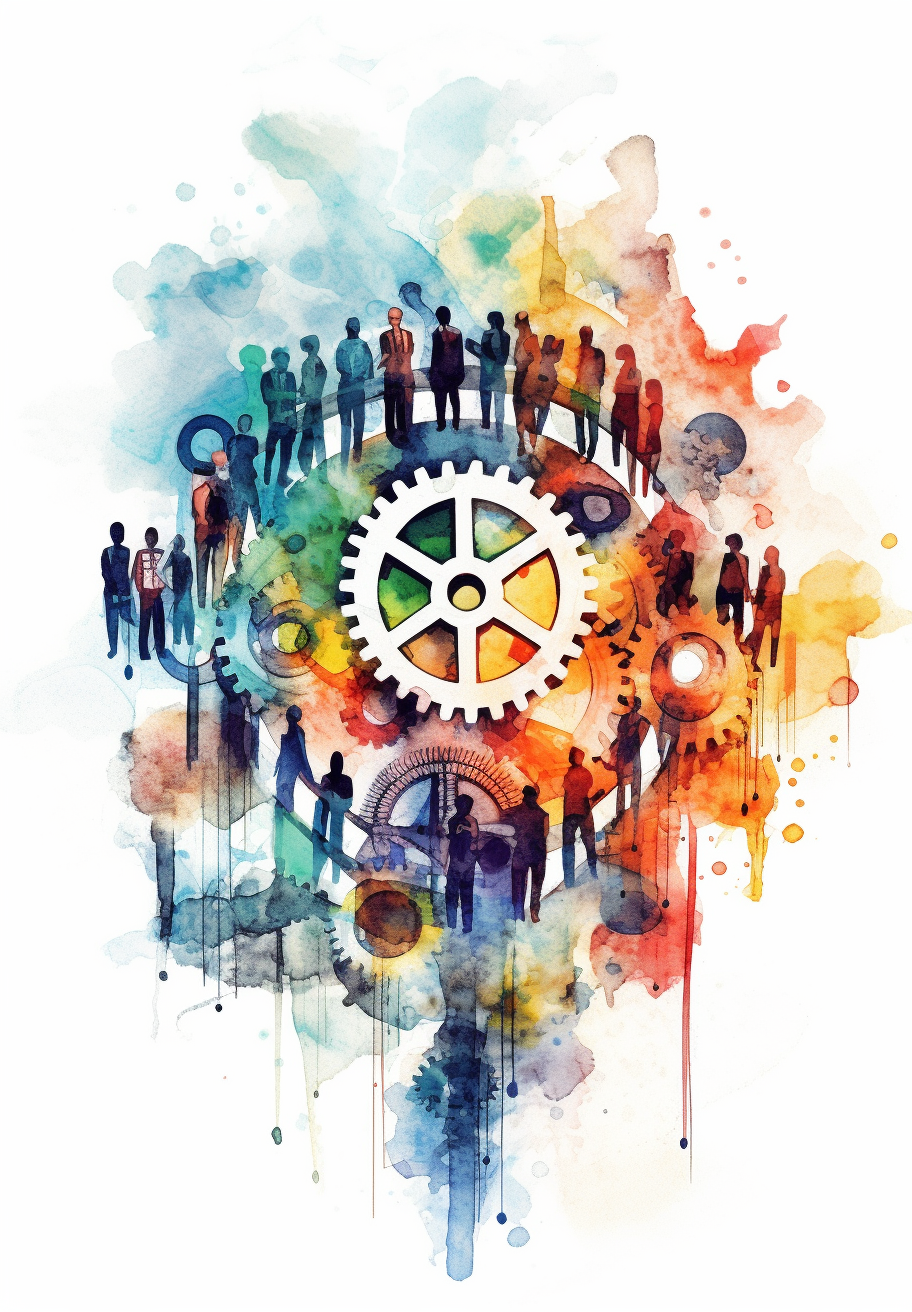
\includegraphics[keepaspectratio, width=\textwidth, height=\textheight]{images/07be4a47-3beb-4a74-a68f-7c7382e8930f.png}
    \caption{Aquarelle représentant différentes manières d'organiser différentes équipes.\\
        Image générée par Kevin Delfour sur Midjourney.}
\end{figure}
\newpage

\chapter{Les alternatives au modèle d'entreprise libérée}

Alors que le modèle d'entreprise libérée a certainement sa place dans le panorama contemporain du management, il serait réducteur de l'ériger comme la seule voie vers un environnement de travail plus égalitaire, autonome et épanouissant. En effet, une pléthore d'autres formes d'organisation et de management existent, chacune offrant ses propres avantages et inconvénients, ainsi que ses propres réponses à la question de l'autonomie, de la participation et du bien-être des employés. Cela illustre bien l'idée que le management est un domaine dynamique, innovant et diversifié, où de nouvelles idées et approches sont constamment explorées et mises en pratique\footnote{Cunliffe, A. L. (2009). The philosopher leader: On relationalism, ethics and reflexivity—a critical perspective to teaching leadership. Management Learning, 40(1), 87-101.}.

\section{Les autres formes d'organisation et de management}

De nombreuses autres formes d'organisation et de management cherchent à redéfinir la relation entre les employés et leurs lieux de travail, en se concentrant sur l'autonomie, la participation, le bien-être et la performance. Elles offrent des alternatives intéressantes au modèle d'entreprise libérée.

\subsection{L'autogestion}

L'autogestion est une forme d'organisation où les employés contrôlent directement et collectivement leur lieu de travail\footnote{Rothschild, J., \& Whitt, J. A. (1986). The cooperative workplace. Cambridge University Press.}. Ce type de structure est souvent utilisé dans les coopératives de travailleurs, où les employés sont également propriétaires de l'entreprise. Il n'y a pas de gestionnaires au sens traditionnel du terme ; les décisions sont prises démocratiquement, souvent par le biais de réunions de travailleurs.

\subsection{L'entreprise démocratique}

Dans une entreprise démocratique, les employés participent activement aux décisions de l'entreprise. Ce modèle s'inspire des principes démocratiques pour créer une culture d'égalité et de participation\footnote{Semler, R. (2003). The Seven-Day Weekend: Changing the Way Work Works. Portfolio.}. Les employés peuvent voter sur diverses questions, comme la stratégie de l'entreprise, l'allocation des ressources et même la sélection des dirigeants.

\subsection{L'entreprise sociocratique}

La sociocratie est un système de gouvernance basé sur le consentement et l'égalité du pouvoir\footnote{Endenburg, G. (1998). Sociocracy: The organization of decision-making, "no objection!" as the principle of sociocracy. Eburon.}. Elle repose sur des cercles de décision semi-autonomes, où chaque membre a une voix égale dans le processus de prise de décision. Ce modèle vise à faciliter la coopération, l'innovation et le respect au sein de l'entreprise.

Chacune de ces alternatives offre sa propre approche pour créer un environnement de travail plus égalitaire et autonome. Cependant, comme le modèle d'entreprise libérée, elles ne sont pas sans défis et exigent une attention particulière à la mise en œuvre et à la gestion.

\section{Les innovations et les expérimentations en cours}

Dans le monde des affaires dynamique et en constante évolution d'aujourd'hui, de nombreuses entreprises cherchent à repousser les limites de ce qui est possible en matière d'organisation et de management. Ces expérimentations, souvent guidées par des principes d'agilité, de responsabilité et d'autonomie, peuvent offrir des aperçus intéressants de l'avenir du travail.

L'une de ces innovations est le concept d'entreprise teal, popularisé par Frédéric Laloux dans son livre "Reinventing Organizations"\footnote{Laloux, F. (2014). Reinventing Organizations. Nelson Parker.}. Les organisations teal se caractérisent par leur autogestion, leur orientation vers la réalisation du potentiel humain et leur vision évolutive du monde.

Une autre tendance notable est l'adoption de modèles d'organisation agiles, en particulier dans le secteur de la technologie. Ces modèles sont axés sur la réactivité, la flexibilité et la collaboration, avec des équipes autogérées qui travaillent sur des projets en cycles courts et itératifs.

Enfin, certains suggèrent que le futur du travail pourrait être caractérisé par des organisations plus distribuées et décentralisées, avec des équipes de travail dispersées géographiquement et une plus grande utilisation des technologies numériques pour la collaboration\footnote{Hinds, P. J., \& Kiesler, S. (Eds.). (2002). Distributed work. MIT Press.}.

Chacune de ces expérimentations offre une perspective unique sur la manière dont les organisations pourraient évoluer à l'avenir. Cependant, il est important de noter que ces innovations sont encore en cours d'exploration et de développement, et que leurs implications à long terme restent incertaines.

\section{Les perspectives d'évolution du modèle d'entreprise libérée}

Le modèle d'entreprise libérée, malgré les critiques et les défis qu'il a rencontrés, est loin d'être figé. De nombreuses entreprises qui ont adopté ce modèle continuent de l'adapter et de l'évoluer en fonction de leurs besoins spécifiques, de leurs expériences et des retours de leurs employés.

Il est probable que nous verrons de nombreuses variations sur le thème de l'entreprise libérée dans les années à venir. Certaines entreprises pourraient chercher à fusionner le modèle d'entreprise libérée avec d'autres approches de management, créant ainsi des hybrides uniques qui combinent le meilleur de plusieurs mondes. Par exemple, l'idée d'une entreprise libérée pourrait être combinée avec les principes de l'agilité, créant une organisation qui est non seulement autonome, mais aussi hautement réactive et adaptable\footnote{Denning, S. (2018). Age of Agile. Amacom.}.

D'autres pourraient chercher à appliquer les principes de l'entreprise libérée à différents niveaux de l'organisation, créant ainsi des "îlots de liberté" au sein de structures plus traditionnelles. Cela pourrait permettre une plus grande expérimentation et adaptation, tout en minimisant les risques associés à une transformation complète de l'entreprise\footnote{Getz, I. (2011). Freedom, Inc.: Free Your Employees and Let Them Lead Your Business for Greater Success. Crown Business.}.

Dans tous les cas, il est clair que le modèle d'entreprise libérée a stimulé une réflexion importante sur la manière dont les entreprises sont gérées et organisées. Il continuera probablement à influencer le discours et la pratique du management dans un avenir proche, même si sa forme et son application peuvent évoluer.


    % Part 04
    \part{L'expérience humaine dans les entreprises libérées}

Jusqu'ici, nous avons parlé du modèle. Il est temps de parler des gens.

Parce qu'une entreprise libérée, vue de l'intérieur, ce n'est pas un schéma d'organisation : c'est un quotidien. Celui du salarié qui découvre l'autonomie — et parfois son vertige. Celui du dirigeant qui doit détenir le pouvoir sans s'en servir, tous les jours, y compris les mauvais. Celui du client, du fournisseur, du territoire, qui traitent avec une entreprise devenue étrange à leurs yeux.

Cette quatrième partie est celle qui porte le mieux le titre du livre : c'est ici qu'on regarde l'envers du décor humain — les épanouissements réels et les souffrances réelles, sans sacrifier les uns aux autres.

Une règle d'honnêteté pour la traverser : les enthousiastes et les déçus ont existé dans les mêmes entreprises, aux mêmes époques. Toute version de l'histoire qui efface l'un des deux camps est une version fausse.


    % Chapter 01
    \insertImage{1d19cb7a-fad3-43c3-b5ed-42e53fc67784.png}{Aquarelle représentant diverses personnes dans un environnement professionnel dynamique et transparent. Leurs expressions sont satisfaites et épanouies, symbolisant leurs expériences positives.}

\chapter{Les expériences des employés}

\lettrine[lines=2]{J}{usqu'ici}, nous avons parlé structures, décisions, indicateurs. Il est temps de parler des seules personnes sans qui tout ça n'est que de la théorie d'organisation : celles qui vivent le modèle du lundi au vendredi.

Et je veux poser une règle pour ce chapitre : on écoute tout le monde. Pas seulement les enthousiastes qu'on fait monter sur scène dans les conférences, mais aussi ceux pour qui la libération a été une épreuve. Un livre qui s'appelle « l'envers du décor » et qui ne raconterait que des épanouissements ne vaudrait pas mieux que les plaquettes qu'il prétend dépasser.

\section{L'impact de l'autonomie sur l'engagement des employés}

Commençons par ce qui est solide : le lien entre autonomie et engagement n'est pas un slogan de consultant, c'est l'un des résultats les mieux établis de la psychologie du travail. Quand les gens contrôlent la manière dont ils font leur travail, leur motivation et leur implication augmentent — la recherche le mesure depuis des décennies\footnote{Langfred, C. W., \& Moye, N. A. (2004). Effects of task autonomy on performance: an extended model considering motivational, informational, and structural mechanisms. Journal of Applied Psychology, 89(6), 934-945.}.

Le terrain le confirme. Chez Chrono Flex, les techniciens itinérants ont reçu le pouvoir de décider sur place, chez le client, sans remonter la chaîne — et leur dirigeant décrit un effet immédiat sur la réactivité comme sur la fierté du métier\footnote{Gérard, A. (2017). Le patron qui ne voulait plus être chef. Flammarion.}. Rien de mystérieux là-dedans : être traité en adulte donne envie de se comporter en adulte. C'est toute la thèse du modèle, et sur ce point, elle tient.

Mais l'autonomie a une face B, et il faut la dire avec la même netteté : l'autonomie est une charge. Décider, c'est porter la décision. Là où l'organisation classique offrait le confort discret de la non-responsabilité — « je n'ai fait qu'appliquer » —, l'entreprise libérée expose chacun aux conséquences de ses choix. Pour certains, c'est grisant. Pour d'autres, c'est une source d'anxiété permanente, d'autant plus difficile à avouer que l'enthousiasme est devenu la norme sociale de l'entreprise. Quand « être autonome » est la valeur cardinale, dire « je suis perdu » devient un aveu coûteux.

Et il y a les préférences, tout simplement. Certains veulent un cadre, des attentes claires, une frontière nette entre le travail et la maison — et font par ailleurs un travail remarquable. Une entreprise libérée qui traite ces profils comme des salariés de seconde zone fabrique de la souffrance avec les meilleures intentions du monde. L'autonomie devrait être une offre. Malheur à ceux qui en font une injonction.

\section{Gestion des défis et des conflits dans un environnement de travail libéré}

Reprenons la question du conflit, mais cette fois du point de vue de celui qui le vit.

Vous êtes en désaccord profond avec un collègue — sur une décision, une répartition de la charge, une attitude. Dans une organisation classique, vous savez à qui en parler, même si vous savez aussi que ce sera imparfait. Dans une entreprise libérée mal outillée, vous êtes seul face à une question vertigineuse : à qui je m'adresse ? Il n'y a pas de chef. Aller voir l'équipe, c'est transformer un différend en tribunal. Ne rien dire, c'est laisser pourrir. La transparence, si fière d'elle-même, fait le reste : tout le monde voit tout, y compris vos tensions.

Ajoutez le problème de la décision évitée : quand personne n'a clairement l'autorité, certaines décisions inconfortables — recadrer un comportement, arrêter un projet auquel un collègue tient — ne sont prises par personne\footnote{Hollander, E. P. (1992). Leadership, followership, self, and others. Leadership Quarterly, 3(1), 43-54.}. Chacun attend que quelqu'un d'autre ose. Dans le vocabulaire des développeurs, c'est un deadlock : tout le monde attend tout le monde.

Les entreprises libérées matures répondent par des mécanismes explicites, et on retrouve ceux du chapitre sur les ressources humaines — médiation par les pairs, escalade progressive définie à l'avance, rôles de facilitation\footnote{Laloux, F. (2014). Reinventing Organizations: A Guide to Creating Organizations Inspired by the Next Stage of Human Consciousness. Nelson Parker.}. Je n'y reviens pas, sauf pour insister sur le point de vue du salarié : ce qui compte pour lui, ce n'est pas l'élégance du mécanisme, c'est de savoir \emph{avant d'en avoir besoin} qu'il existe, comment il marche, et qu'il peut s'en saisir sans être étiqueté fauteur de trouble. Un processus de médiation que personne n'ose déclencher est un poster de plus dans le hall.

\section{Ce que disent ceux qui y travaillent}

Je dois vous faire un aveu d'auteur : les « témoignages » qu'on lit dans la littérature sur les entreprises libérées — y compris dans la première version de ce chapitre — sont presque toujours de seconde main, souvent lissés, parfois inventés. J'ai décidé de ne pas jouer à ce jeu-là. Voici ce qu'on sait vraiment, et d'où on le sait.

Ce qu'on sait des enthousiasmes est bien documenté par ceux qui ont raconté leur transformation de l'intérieur. Les récits de FAVI rapportent des opérateurs fiers de gérer leur production et attachés à leur autonomie au point qu'un retour en arrière semblait impensable\footnote{Zobrist, J.-F. (2012). La belle histoire de FAVI: L'entreprise qui croit que l'homme est bon. Humanisme \& Organisations.}. Chez Chrono Flex, Alexandre Gérard décrit des équipes transformées par la confiance reçue — et ne cache d'ailleurs pas les turbulences du chemin\footnote{Gérard, A. (2017). Le patron qui ne voulait plus être chef. Flammarion.}.

Ce qu'on sait des difficultés est plus dispersé, parce que les déçus n'écrivent pas de livres : surcharge de réunions et de rôles chez les uns, anxiété de la responsabilité chez d'autres, sentiment d'un pouvoir devenu informel — donc inattaquable — chez d'autres encore. Ces récits-là, on les recueille en off.

Et puis il y a ce que j'ai entendu moi-même, dans les circonstances les plus honnêtes qui soient : la liquidation de ma propre société — j'y reviendrai dans la conclusion de ce livre. Quand une entreprise ferme, plus personne n'a de raison d'enjoliver quoi que ce soit ; ce qui se dit à ce moment-là, c'est la vérité résiduelle. Voici ce que mes collaborateurs m'ont dit en partant.

Plusieurs m'ont confié qu'ils allaient chercher ailleurs en sachant qu'ils ne retrouveraient jamais ce cadre-là — la pire des publicités pour le marché du travail, la meilleure pour le modèle. D'autres, plus jeunes, m'ont dit vouloir rejoindre des entreprises classiques, précisément pour comprendre ce qu'ils perdraient au change — et j'ai trouvé cette lucidité magnifique : on ne mesure une liberté qu'en la quittant. Et certains m'ont dit, sans détour, que trop de responsabilités, ce n'était pas pour eux.

Trois réactions, un seul modèle. Les trois sont vraies en même temps, et aucune n'annule les autres : c'est exactement ça, l'expérience des employés d'une entreprise libérée. Un salarié épanoui par l'autonomie et un salarié épuisé par elle peuvent travailler dans la même entreprise, la même année, au même étage. Tant qu'on n'accepte pas que ces deux vérités coexistent, on ne comprend rien à ce chapitre — ni à ce livre.

    % Chapter 03
    \insertImage{a1837c37-748e-4d37-8201-7339d1d76a59.png}{Aquarelle représentant des leaders aux côtés de leurs employés dans un environnement de travail collaboratif.}

\chapter{Le rôle des leaders dans les entreprises libérées}

Lorsqu'on parle d'entreprises libérées, on a souvent l'impression que la hiérarchie disparaît complètement. Cependant, même si les entreprises libérées cherchent à aplanir la hiérarchie et à décentraliser le pouvoir, cela ne signifie pas que le leadership n'est plus nécessaire. Au contraire, le rôle du leader dans une entreprise libérée est crucial, mais il peut être très différent de ce que nous voyons dans des organisations plus traditionnelles.

Dans ce chapitre, nous allons explorer le rôle des leaders dans les entreprises libérées, comment ils contribuent à la réussite de l'entreprise, les défis auxquels ils sont confrontés et les récompenses qu'ils peuvent récolter. Nous partagerons également des témoignages et des études de cas de leaders qui ont réussi à naviguer dans le monde complexe et parfois déroutant de l'entreprise libérée.

L'objectif de ce chapitre est de montrer que, bien que les entreprises libérées puissent nécessiter un style de leadership différent, elles n'éliminent pas le besoin de leaders forts et efficaces.

\section{Redéfinir le leadership dans une entreprise libérée}

Dans une entreprise libérée, le rôle du leader est profondément transformé. Au lieu de contrôler et de diriger, les leaders sont là pour servir de catalyseurs et de facilitateurs. Ils créent un environnement où les employés peuvent s'épanouir, apporter leurs propres idées et prendre des initiatives.

Dans ce contexte, le leadership ne se limite pas à une position hiérarchique. Il s'agit davantage d'une compétence qui peut être exercée par n'importe qui, à n'importe quel niveau de l'organisation. C'est ce qu'on appelle parfois le "leadership distribué"\footnote{Bolden, R. (2011). Distributed leadership in organizations: A review of theory and research. International Journal of Management Reviews, 13(3), 251-269.}.

Cela signifie que le rôle des leaders formels - comme les managers et les dirigeants - change considérablement. Au lieu de prendre toutes les décisions et de dicter ce que les autres doivent faire, ils sont là pour soutenir et habilité leurs collègues. Ils servent de guides et de mentors, aidant les autres à développer leurs propres capacités de leadership.

Par exemple, chez Michelin, un fabricant de pneus français qui a adopté le modèle d'entreprise libérée, les managers ne sont plus considérés comme des chefs, mais comme des "leaders-coachs". Leur rôle est de favoriser l'autonomie et l'engagement des employés, en fournissant un soutien et des conseils, plutôt que des ordres\footnote{Getz, I. (2009). Liberation management: necessary disorganization for the nanosecond nineties. Michelin.}.

Dans l'ensemble, le leadership dans une entreprise libérée est moins une question de pouvoir et de contrôle, et plus une question de service et d'autonomisation.

\section{Défis et récompenses du leadership libéré}

Devenir un leader dans une entreprise libérée peut être à la fois gratifiant et difficile. Commençons par les défis.

Les leaders dans les entreprises libérées doivent souvent lutter contre des décennies de conditionnement sur ce que signifie être un leader. Ils doivent abandonner l'idée que le leader est celui qui contrôle et décide de tout. Cela peut être déstabilisant et même effrayant pour certains.

De plus, en tant que facilitateur plutôt que décideur, le leader doit souvent faire face à des dilemmes et des paradoxes. Par exemple, comment intervenir dans un conflit sans prendre le contrôle ? Comment aider une équipe à atteindre ses objectifs sans imposer sa vision ? Ces questions ne sont pas faciles à résoudre et nécessitent une grande dose de sagesse et d'humilité.

Malgré ces défis, être un leader dans une entreprise libérée peut aussi être extrêmement gratifiant.

D'abord, il y a la satisfaction de voir les employés s'épanouir et prendre des initiatives. De nombreux leaders rapportent qu'il est très gratifiant de voir leurs collègues grandir et s'épanouir dans un environnement de travail libéré\footnote{Laloux, F. (2014). Reinventing organizations: A guide to creating organizations inspired by the next stage of human consciousness. Nelson Parker.}.

Ensuite, il y a le plaisir de contribuer à quelque chose de plus grand que soi. Les entreprises libérées cherchent souvent à avoir un impact positif non seulement sur leurs employés et leurs clients, mais aussi sur la société dans son ensemble. En tant que leader, vous pouvez jouer un rôle clé dans la réalisation de cette vision.

Enfin, il y a la possibilité d'apprendre et de grandir en tant que personne. Le voyage vers le leadership libéré est souvent un voyage de développement personnel, où vous êtes amené à questionner vos croyances et vos habitudes, à apprendre de nouvelles compétences et à devenir une meilleure version de vous-même.

\section{Témoignages de leaders et études de cas}

Pour illustrer le rôle des leaders dans les entreprises libérées, voici quelques témoignages et études de cas de leaders qui ont réussi à naviguer dans le monde complexe et parfois déroutant de l'entreprise libérée.

\subsection{Témoignage 1 : Un leader chez Poult}

Poult, le fabricant de biscuits français que nous avons mentionné précédemment, est dirigé par une équipe de leaders qui se considèrent davantage comme des "facilitateurs" que comme des "chefs". Un de ces leaders partage son expérience :

"En tant que leader chez Poult, mon rôle est de soutenir mes collègues et de leur donner les moyens de réussir. Cela peut être difficile parfois, car je dois résister à l'envie de prendre le contrôle et de résoudre les problèmes moi-même. Mais quand je vois comment les gens s'épanouissent et prennent des initiatives, je sais que cela en vaut la peine"\footnote{Rodriguez, B. (2014). Poult. L'Usine nouvelle.}.

\subsection{Témoignage 2 : Un leader chez FAVI}

FAVI, la fonderie française, est dirigée par une équipe de leaders qui croient fermement à l'autonomie et à la responsabilisation. Un de ces leaders décrit son expérience comme suit :

"Chez FAVI, je suis moins un manager qu'un coach. Mon rôle est d'aider mes collègues à développer leurs compétences et à prendre des décisions. C'est un défi constant, car chaque personne est unique et a ses propres besoins. Mais c'est aussi extrêmement gratifiant de voir les gens grandir et devenir plus confiants et autonomes"\footnote{Getz, I. (2009). Liberation management: necessary disorganization for the nanosecond nineties. Favi S.A.}.

Ces témoignages montrent que le leadership dans une entreprise libérée peut être à la fois un défi et une source d'épanouissement personnel et professionnel.

    % Chapter 03
    \insertImage{4d3ea27d-bc3c-4d12-999c-9c5b794ad904.png}{Aquarelle représentant diverses parties prenantes en cercle autour d'une personne inspirante représentant une entreprise libérée.}

\chapter{Les impacts sur les parties prenantes externes}

Une entreprise libérée adore parler d'elle-même — c'est presque un symptôme. Ses équipes, ses rituels, sa culture, sa transformation. Mais aucune entreprise ne vit en vase clos : il y a des clients qui appellent, des fournisseurs qui livrent, des partenaires qui signent, et un territoire qui regarde tout ça d'un œil parfois perplexe.

Ce chapitre sort donc des murs. Que voit-on de l'extérieur quand une entreprise se libère ? Et qu'est-ce que ça change, concrètement, pour ceux qui traitent avec elle ?

\section{Relation avec les clients dans une entreprise libérée}

Pour un client, une entreprise libérée se reconnaît à un détail qui change tout : la personne en face de vous peut dire oui.

Dans une organisation classique, le premier interlocuteur est rarement le décideur — il transmet, il escalade, il revient vers vous. Dans une entreprise libérée, celui qui traite votre problème a le pouvoir de le résoudre. Chez Chrono Flex, c'est le cœur du réacteur : le technicien qui intervient sur votre chantier décide sur place, sans appeler un bureau\footnote{Gérard, A. (2017). Le patron qui ne voulait plus être chef. Flammarion.}. Pour le client pressé — et dans le dépannage hydraulique, le client est toujours pressé —, la différence se mesure en heures de production sauvées.

Chez FAVI, la logique était poussée jusqu'à l'architecture même de l'entreprise : des mini-usines dédiées chacune à un client, avec un contact direct entre les opérateurs et « leur » client\footnote{Getz, I. (2009). Liberating Leadership: How the Initiative-Freeing Radical Organizational Form Has Been Successfully Adopted. California Management Review, 51(4), 32-58.}. L'ouvrier qui coule le laiton sait pour qui il le coule. Difficile de faire plus court comme circuit qualité.

Soyons complets : ce niveau de personnalisation a ses fragilités. Il dépend de la constance des équipes — un client habitué à l'excellence pardonne mal les jours sans. Et certains clients, notamment les grandes organisations, sont déroutés par l'absence d'interlocuteur hiérarchique : « qui est le responsable ? » n'est pas toujours une question de méfiance, c'est parfois juste une case obligatoire de leur processus achats. Une entreprise libérée doit apprendre à répondre à cette question sans renier son modèle — généralement en désignant des référents, ce qui n'est pas la même chose que des chefs.

\section{Relation avec les fournisseurs et les partenaires commerciaux}

La libération déborde naturellement sur la chaîne de valeur, pour une raison de simple cohérence : on ne peut pas prôner la confiance en interne et pressurer ses fournisseurs comme au bon vieux temps.

Les entreprises libérées tendent donc vers des relations de partenariat plutôt que des rapports de force : transparence sur les contraintes, co-construction des solutions, engagement dans la durée. Ce n'est pas de l'angélisme — c'est le même pari que le modèle fait en interne, appliqué à l'externe : la confiance coûte moins cher que le contrôle, à condition d'être réciproque.

Mais la réciprocité, justement, ne se décrète pas plus dehors que dedans. Tous les fournisseurs ne veulent pas « co-construire » — certains veulent un bon de commande précis et être payés à l'heure, et c'est une position parfaitement respectable. Et tous les partenaires ne jouent pas le jeu : la transparence unilatérale, face à un acheteur resté à l'ancienne école, peut devenir un handicap de négociation. Comme pour les salariés, la règle devrait être la même : le partenariat est une offre, pas une imposition.


\section{Impact sur la communauté locale et la société}

C'est peut-être l'effet le moins commenté et le plus profond du modèle : ce qu'une entreprise libérée fait au territoire qui l'entoure.

L'exemple le plus parlant reste FAVI, et il ne s'agit pas d'une opération de mécénat. Pendant que la sous-traitance automobile délocalisait en masse, FAVI est restée à Hallencourt, village picard de quelques centaines d'habitants, en faisant le pari que des équipes responsabilisées seraient plus compétitives que des coûts salariaux réduits\footnote{Getz, I. (2009). Liberating Leadership: How the Initiative-Freeing Radical Organizational Form Has Been Successfully Adopted. California Management Review, 51(4), 32-58.}. Pour un territoire rural, une entreprise industrielle qui reste — et qui embauche —, c'est un impact social qui se passe de discours.

Il y a aussi un effet plus diffus, que je crois réel même s'il est difficile à mesurer : des gens qui apprennent au travail à décider, à se coordonner sans chef, à porter des responsabilités, ne redeviennent pas passifs en franchissant la porte de l'entreprise. Le travail est une école — la question est seulement de savoir ce qu'il enseigne. Une organisation qui enseigne l'initiative et la coopération rend à la société des citoyens un peu différents de celle qui enseigne l'obéissance et la prudence.

Gardons-nous cependant d'un raccourci : « libérée » ne veut pas dire « vertueuse ». Une entreprise peut être libérée et polluer, être libérée et vendre n'importe quoi. L'engagement sociétal et environnemental est un choix distinct, qui demande ses propres preuves. Inversement, des organisations qui ne se revendiquent pas du modèle — je pense aux coopératives, dont le pouvoir partagé est inscrit dans les statuts mêmes — produisent depuis longtemps des effets sociaux comparables sans jamais employer le mot « libération »\footnote{Rothschild, J., \& Whitt, J. A. (1986). The cooperative workplace. Cambridge University Press.}. Le modèle n'a pas le monopole du sens.

Au fond, la question que ce chapitre pose aux dirigeants tentés par la libération est celle-ci : pour qui libérez-vous ? Si la réponse s'arrête aux murs de l'entreprise, vous passez à côté de la moitié de l'histoire.



% Back matter
\backmatter

    % Conclusion
    \part*{Conclusion}
\addcontentsline{toc}{part}{Conclusion}
\insertImage{0411efc2-c833-43fb-9675-cb74860ca78d.png}{Aquarelle d'une route ouverte traversant un désert avec une ville moderne au bout de la route, symbolisant les perspectives d'évolution des sociétés libérées.}

Au début de ce livre, je vous ai promis l'envers du décor. Nous y sommes allés : les décisions qui n'aboutissent pas, les managers à qui on retire leur métier, les salariés épuisés par une autonomie qu'ils n'avaient pas demandée, les libérations de façade, les sources embellies, les échecs qu'on ne raconte jamais sur scène.

Et voici l'aveu final : après tout ça, je crois toujours à ce modèle. Peut-être même davantage qu'avant — mais plus de la même façon. Laissez-moi vous expliquer ce qui a changé, et ce que j'en retire pour la suite.

\section*{Les enseignements à tirer pour les entreprises libérées et les autres organisations}

Si je devais compresser ce livre en trois leçons, voici celles que je garderais.

\textbf{La confiance fonctionne — mais c'est une construction, pas une déclaration.} Partout où le modèle réussit, on retrouve le même schéma : des années de gestes cohérents qui prouvent que la confiance est réelle, des équipes formées avant d'être responsabilisées, une transparence qui rend l'autonomie praticable. Et partout où il échoue, le symétrique : une liberté annoncée un lundi matin, plaquée sur une organisation qu'on n'a ni écoutée ni préparée. Le modèle ne pardonne pas la précipitation — c'est peut-être sa caractéristique la plus constante.

\textbf{Ce qu'on supprime compte moins que ce qu'on construit à la place.} La hiérarchie rendait des services invisibles : aligner, arbitrer, protéger, faire circuler l'information. Une libération sérieuse commence par l'inventaire de ces services et par la conception de ce qui les remplacera — rituels de décision, mécanismes de résolution des conflits, dispositifs de protection des personnes. Celle qui saute cette étape n'obtient pas la liberté : elle obtient du flou, et le flou profite toujours aux plus forts.

\textbf{L'envers du décor est humain, pas organisationnel.} La vraie zone d'ombre du modèle, celle qui m'a poussé à écrire, n'est pas dans les organigrammes : elle est dans le surmenage de ceux qui n'arrivent pas à poser leurs limites, dans l'injonction à l'enthousiasme, dans le pouvoir informel qui ne se voit pas donc ne se conteste pas. Une entreprise libérée honnête se juge à sa capacité à regarder ces risques en face et à s'outiller contre eux — pas à la beauté de son discours.

Ces leçons dépassent d'ailleurs le modèle. Même si vous ne libérez jamais votre entreprise, les questions qu'il pose — qui décide, qui sait, qui est protégé, qui grandit — méritent d'être posées dans n'importe quelle organisation. C'est le grand mérite du mouvement : avoir remis ces questions sur la table.

\section*{Les pistes de réflexion pour l'avenir}

Et maintenant ? Trois convictions pour la route.

\textbf{L'avenir appartient aux hybrides.} La grande bascule romantique — toute l'entreprise, d'un coup, pour toujours — restera l'exception. Ce qui se diffuse, ce sont des combinaisons pragmatiques : des îlots de liberté dans des groupes classiques, des gouvernances explicites héritées de la sociocratie, une transparence économique devenue banale. Les puristes y verront une trahison. J'y vois le signe qu'un modèle devient adulte : il accepte d'être adapté plutôt qu'adoré.

\textbf{La prochaine frontière est celle des garde-fous.} La première génération d'entreprises libérées a démontré que la confiance pouvait fonctionner. La suivante devra démontrer qu'elle peut fonctionner \emph{pour tout le monde} : protéger les discrets autant que les audacieux, offrir l'autonomie sans l'imposer, rendre le pouvoir informel visible et contestable. Le modèle a gagné le débat de l'efficacité ; il lui reste à gagner celui de la justice. C'est un chantier plus difficile — et plus important.

\textbf{Le mot disparaîtra peut-être ; les questions resteront.} Les modes managériales passent, et « entreprise libérée » subira peut-être le sort de tous les étendards. Peu importe, sincèrement. Si dans vingt ans plus personne n'emploie l'expression parce que la confiance par défaut, la décision au plus près du terrain et le manager-jardinier sont devenus des évidences, le mouvement aura réussi au-delà de toute espérance. On ne mesure pas une idée à la longévité de son nom, mais à ce qu'elle laisse dans les pratiques.

% [KEVIN : c'est ici que le livre attend TA conclusion personnelle — où en es-tu, toi, après ce voyage ? Que dirais-tu au Kevin d'il y a quelques années qui découvrait le modèle ? Quelques paragraphes à la première personne feraient la vraie fin de ce livre.]

Une dernière chose. Si vous refermez ce livre en vous disant « c'est décidément trop risqué », j'aurai à moitié échoué. Si vous le refermez en vous disant « c'est facile, lançons-nous », j'aurai complètement échoué. La bonne sortie, c'est celle du randonneur qui a lu la carte : vous connaissez maintenant les gouffres, les rivières à crocodiles et les faux raccourcis. Le sommet, lui, n'a pas bougé.

Il n'attend que des gens lucides pour y monter. Bonne route.


    % Remerciements
    \part*{Remerciements}
\addcontentsline{toc}{part}{Remerciements}
\markboth{}{}

Je tiens à exprimer ma gratitude profonde à tous ceux qui ont rendu ce livre possible.

En premier lieu, merci à toutes les entreprises libérées qui ont partagé leurs expériences, leurs succès et leurs défis. Vos histoires ont enrichi ce livre et ont ajouté une précieuse dimension pratique à notre exploration de ce modèle d'entreprise fascinant.

Je tiens également à remercier les nombreux chercheurs et penseurs qui ont étudié et écrit sur le sujet des entreprises libérées. Vos travaux ont fourni un cadre solide pour notre compréhension de ce phénomène et ont éclairé de nombreuses aspects de notre discussion.

Un merci tout particulier à ma famille et mes amies pour leur soutien constant, leurs conseils précieux et leur patience infinie tout au long de ce processus d'écriture. Vous avez rendu ce voyage beaucoup plus agréable et enrichissant.

Enfin, je tiens à exprimer ma reconnaissance à vous, chers lecteurs, pour votre curiosité et votre intérêt pour ce sujet. J'espère que ce livre vous inspirera à repenser vos propres pratiques managériales et à explorer de nouvelles possibilités pour votre organisation.


    \newpage

    \listoffigures

    \newpage
    
    \listoffootnotes 
    
    \newpage
    \thispagestyle{empty}
    \mbox{}

% Fin du document
\end{document}
